% ------------------------------------------------------------
% LaTeX Template für die DHBW zum Schnellstart!
% Original: https://github.wdf.sap.corp/vtgermany/LaTeX-Template-DHBW
% ------------------------------------------------------------
% ---- Präambel mit Angaben zum Dokument
\documentclass[
	fontsize=12pt,           % Leitlinien sprechen von Schriftgröße 12.
	paper=A4,
	twoside=false,
	listof=totoc,            % Tabellen- und Abbildungsverzeichnis ins Inhaltsverzeichnis
	bibliography=totoc,      % Literaturverzeichnis ins Inhaltsverzeichnis aufnehmen
	titlepage,               % Titlepage-Umgebung anstatt \maketitle
	headsepline,             % horizontale Linie unter Kolumnentitel
	abstracton,              % Überschrift einschalten, Abstract muss in {abstract}-Umgebung stehen
]{scrreprt}                  % Verwendung von KOMA-Report
\usepackage[utf8]{inputenc}  % UTF8 Encoding einschalten
\usepackage[ngerman]{babel}  % Neue deutsche Rechtschreibung
\usepackage[T1]{fontenc}     % Ausgabe von westeuropäischen Zeichen (auch Umlaute)
\usepackage{microtype}       % Trennung von Wörtern wird besser umgesetzt
\usepackage{lmodern}         % Nicht-gerasterte Schriftarten (bei MikTeX erforderlich)
\usepackage{graphicx}        % Einbinden von Grafiken erlauben
\usepackage{wrapfig}         % Grafiken fließend im Text
\usepackage{setspace}        % Zeilenabstand \singlespacing, \onehalfspaceing, \doublespacing
\usepackage[
	%showframe,                % Ränder anzeigen lassen
	left=2.7cm, right=2.5cm,
	top=2.5cm,  bottom=2.5cm,
	includeheadfoot
]{geometry}                      % Seitenlayout einstellen
\usepackage{scrlayer-scrpage}    % Gestaltung von Fuß- und Kopfzeilen
\usepackage{acronym}             % Abkürzungen, Abkürzungsverzeichnis
\usepackage{titletoc}            % Anpassungen am Inhaltsverzeichnis
\contentsmargin{0.75cm}          % Abstand im Inhaltsverzeichnis zw. Punkt und Seitenzahl
\usepackage[                     % Klickbare Links (enth. auch "nameref", "url" Package)
  hidelinks,                     % Blende die "URL Boxen" aus.
  breaklinks=true                % Breche zu lange URLs am Zeilenende um
]{hyperref}
\usepackage[hypcap=true]{caption}% Anker Anpassung für Referenzen
\urlstyle{same}                  % Aktuelle Schrift auch für URLs
% Anpassung von autoref für Gleichungen (ergänzt runde Klammern) und Algorithm.
% Anstatt "Listing" kann auch z.B. "Code-Ausschnitt" verwendet werden. Dies sollte
% jedoch synchron gehalten werden mit \lstlistingname (siehe weiter unten).
\addto\extrasngerman{%
	\def\equationautorefname~#1\null{Gleichung~(#1)\null}
	\def\lstnumberautorefname{Zeile}
	\def\lstlistingautorefname{Listing}
	\def\algorithmautorefname{Algorithmus}
	% Damit einheitlich "Abschnitt 1.2[.3]" verwendet wird und nicht "Unterabschnitt 1.2.3"
	% \def\subsectionautorefname{Abschnitt}
}

% ---- Abstand verkleinern von der Überschrift 
\renewcommand*{\chapterheadstartvskip}{\vspace*{.5\baselineskip}}

% Hierdurch werden Schusterjungen und Hurenkinder vermieden, d.h. einzelne Wörter
% auf der nächsten Seite oder in einer einzigen Zeile.
% LaTeX kann diese dennoch erzeugen, falls das Layout ansonsten nicht umsetzbar ist.
% Diese Werte sind aber gute Startwerte.
\widowpenalty10000
\clubpenalty10000

% ---- Für das Quellenverzeichnis
\usepackage[
	backend = biber,                % Verweis auf biber
	language = auto,
	style = numeric,                % Nummerierung der Quellen mit Zahlen
	sorting = none,                 % none = Sortierung nach der Erscheinung im Dokument
	sortcites = true,               % Sortiert die Quellen innerhalb eines cite-Befehls
	block = space,                  % Extra Leerzeichen zwischen Blocks
	hyperref = true,                % Links sind klickbar auch in der Quelle
	%backref = true,                % Referenz, auf den Text an die zitierte Stelle
	bibencoding = auto,
	giveninits = true,              % Vornamen werden abgekürzt
	doi=false,                      % DOI nicht anzeigen
	isbn=false,                     % ISBN nicht anzeigen
    alldates=short                  % Datum immer als DD.MM.YYYY anzeigen
]{biblatex}
\addbibresource{Inhalt/literatur.bib}
\setcounter{biburlnumpenalty}{3000}     % Umbruchgrenze für Zahlen
\setcounter{biburlucpenalty}{6000}      % Umbruchgrenze für Großbuchstaben
\setcounter{biburllcpenalty}{9000}      % Umbruchgrenze für Kleinbuchstaben
\DeclareNameAlias{default}{family-given}  % Nachname vor dem Vornamen
\AtBeginBibliography{\renewcommand{\multinamedelim}{\addslash\space
}\renewcommand{\finalnamedelim}{\multinamedelim}}  % Schrägstrich zwischen den Autorennamen
\DefineBibliographyStrings{german}{
  urlseen = {Einsichtnahme:},                      % Ändern des Titels von "besucht am"
}
\usepackage[babel,german=quotes]{csquotes}         % Deutsche Anführungszeichen + Zitate


% ---- Für Mathevorlage
\usepackage{amsmath}    % Erweiterung vom Mathe-Satz
\usepackage{amssymb}    % Lädt amsfonts und weitere Symbole
\usepackage{MnSymbol}   % Für Symbole, die in amssymb nicht enthalten sind.


% ---- Für Quellcodevorlage
\usepackage{scrhack}                    % Hack zur Verw. von listings in KOMA-Script
\usepackage{listings}                   % Darstellung von Quellcode
%\usepackage{xcolor}                     % Einfache Verwendung von Farben
\usepackage[dvipsnames]{xcolor}
% -- Eigene Farben für den Quellcode
\definecolor{JavaLila}{rgb}{0.4,0.1,0.4}
\definecolor{JavaGruen}{rgb}{0.3,0.5,0.4}
\definecolor{JavaBlau}{rgb}{0.0,0.0,1.0}
\definecolor{ABAPKeywordsBlue}{HTML}{6000ff}
\definecolor{ABAPCommentGrey}{HTML}{808080}
\definecolor{ABAPStringGreen}{HTML}{4da619}
\definecolor{PyKeywordsBlue}{HTML}{0000AC}
\definecolor{PyCommentGrey}{HTML}{808080}
\definecolor{PyStringGreen}{HTML}{008080}
% -- Farben für ABAP CDS
\definecolor{CDSString}{HTML}{FF8C00}
\definecolor{CDSKeywords}{HTML}{6000ff}
\definecolor{CDSAnnotation}{HTML}{00BFFF}
\definecolor{CDSComment}{HTML}{808080}
\definecolor{CDSFunc}{HTML}{FF0000}

% -- Default Listing-Styles

\lstset{
	% Das Paket "listings" kann kein UTF-8. Deswegen werden hier 
	% die häufigsten Zeichen definiert (ä,ö,ü,...)
	literate=%
		{á}{{\'a}}1 {é}{{\'e}}1 {í}{{\'i}}1 {ó}{{\'o}}1 {ú}{{\'u}}1
		{Á}{{\'A}}1 {É}{{\'E}}1 {Í}{{\'I}}1 {Ó}{{\'O}}1 {Ú}{{\'U}}1
		{à}{{\`a}}1 {è}{{\`e}}1 {ì}{{\`i}}1 {ò}{{\`o}}1 {ù}{{\`u}}1
		{À}{{\`A}}1 {È}{{\'E}}1 {Ì}{{\`I}}1 {Ò}{{\`O}}1 {Ù}{{\`U}}1
		{ä}{{\"a}}1 {ë}{{\"e}}1 {ï}{{\"i}}1 {ö}{{\"o}}1 {ü}{{\"u}}1
		{Ä}{{\"A}}1 {Ë}{{\"E}}1 {Ï}{{\"I}}1 {Ö}{{\"O}}1 {Ü}{{\"U}}1
		{â}{{\^a}}1 {ê}{{\^e}}1 {î}{{\^i}}1 {ô}{{\^o}}1 {û}{{\^u}}1
		{Â}{{\^A}}1 {Ê}{{\^E}}1 {Î}{{\^I}}1 {Ô}{{\^O}}1 {Û}{{\^U}}1
		{œ}{{\oe}}1 {Œ}{{\OE}}1 {æ}{{\ae}}1 {Æ}{{\AE}}1 {ß}{{\ss}}1
		{ű}{{\H{u}}}1 {Ű}{{\H{U}}}1 {ő}{{\H{o}}}1 {Ő}{{\H{O}}}1
		{ç}{{\c c}}1 {Ç}{{\c C}}1 {ø}{{\o}}1 {å}{{\r a}}1 {Å}{{\r A}}1
		{€}{{\euro}}1 {£}{{\pounds}}1 {«}{{\guillemotleft}}1
		{»}{{\guillemotright}}1 {ñ}{{\~n}}1 {Ñ}{{\~N}}1 {¿}{{?`}}1,
	breaklines=true,        % Breche lange Zeilen um 
	breakatwhitespace=true, % Wenn möglich, bei Leerzeichen umbrechen
	% Symbol für Zeilenumbruch einfügen
	prebreak=\raisebox{0ex}[0ex][0ex]{\ensuremath{\rhookswarrow}},
	postbreak=\raisebox{0ex}[0ex][0ex]{\ensuremath{\rcurvearrowse\space}},
	tabsize=4,                                 % Setze die Breite eines Tabs
	basicstyle=\ttfamily\small,                % Grundsätzlicher Schriftstyle
	columns=fixed,                             % Besseres Schriftbild
	numbers=left,                              % Nummerierung der Zeilen
	%frame=single,                             % Umrandung des Codes
	showstringspaces=false,                    % Keine Leerzeichen hervorheben
	keywordstyle=\color{blue},
	ndkeywordstyle=\bfseries\color{darkgray},
	identifierstyle=\color{black},
	commentstyle=\itshape\color{JavaGruen},   % Kommentare in eigener Farbe
	stringstyle=\color{JavaBlau},             % Strings in eigener Farbe,
	captionpos=b,                             % Bild*unter*schrift
	xleftmargin=5.0ex
}

% ---- Eigener JAVA-Style für den Quellcode
\renewcommand{\ttdefault}{pcr}               % Schriftart, welche auch fett beinhaltet
\lstdefinestyle{EigenerJavaStyle}{
	language=Java,                             % Syntax Highlighting für Java
	%frame=single,                             % Umrandung des Codes
	keywordstyle=\bfseries\color{JavaLila},    % Keywords in eigener Farbe und fett
	commentstyle=\itshape\color{JavaGruen},    % Kommentare in eigener Farbe und italic
	stringstyle=\color{JavaBlau}               % Strings in eigener Farbe
}

% ---- Eigener ABAP-Style für den Quellcode
\renewcommand{\ttdefault}{pcr}
\lstdefinestyle{EigenerABAPStyle}{
	language=[R/3 6.10]ABAP,
	morestring=[b]\|,                          % Für Pipe-Strings
	morestring=[b]\`,                          % für Backtick-Strings
	keywordstyle=\bfseries\color{ABAPKeywordsBlue},
	commentstyle=\itshape\color{ABAPCommentGrey},
	stringstyle=\color{ABAPStringGreen},
	tabsize=2,
	morekeywords={
		types,
		@data,
		as,
		lower,
		start,
		selection,
		order,
		by,
		inner,
		join,
		key,
		end,
		cast
	}
}

% ---- Eigener Python-Style für den Quellcode
\renewcommand{\ttdefault}{pcr}
\lstdefinestyle{EigenerPythonStyle}{
	language=Python,
	columns=flexible,
	keywordstyle=\bfseries\color{PyKeywordsBlue},
	commentstyle=\itshape\color{PyCommentGrey},
	stringstyle=\color{PyStringGreen}
}

%----- ABAP-CDS-View language
\lstdefinelanguage{ABAPCDS}{
	sensitive=false,
	%Keywords
	morekeywords={define,
		view,
		as,
		select,
		from,
		inner,
		join,
		on,
		key,
		case,
		when,
		then,
		else,
		end,
		true,
		false,
		cast,
		where,
		and,
		distinct,
		group,
		by,
		having,
		min,
		sum,
		max,
		count,
		avg
	},
	%Methoden
	morekeywords=[2]{
		div,
		currency\_conversion,
		dats\_days\_between,
		concat\_with\_space,
		dats\_add_days,
		dats\_is\_valid,
		dats\_add\_months,
		unit\_conversion,
		division,
		mod,
		abs,
		floor,
		ceil,
		round,
		concat,
		replace,
		substring,
		left,
		right,
		length
	},
	morecomment=[s][\color{CDSAnnotation}]{@}{:},
	morecomment=[l][\itshape\color{CDSComment}]{//},
	morecomment=[s][\itshape\color{CDSComment}]{/*}{*/},
	morestring=[b][\color{CDSString}]',
	keywordstyle=\bfseries\color{CDSKeywords},
	keywordstyle=[2]\color{CDSFunc}
}

  % Weitere Details sind ausgelagert

\usepackage{algorithm}                  % Für Algorithmen-Umgebung (ähnlich wie lstlistings Umgebung)
\usepackage{algpseudocode}              % Für Pseudocode. Füge "[noend]" hinzu, wenn du kein "endif",
                                        % etc. haben willst.

\makeatletter                           % Sorgt dafür, dass man @ in Namen verwenden kann.
                                        % Ansonsten gibt es in der nächsten Zeile einen Compilefehler.
\renewcommand{\ALG@name}{Algorithmus}   % Umbenennen von "Algorithm" im Header der Listings.
\makeatother                            % Zeichen wieder zurücksetzen
\renewcommand{\lstlistingname}{Listing} % Erlaubt das Umbenennen von "Listing" in anderen Titel.

% ---- Tabellen
\usepackage{booktabs}  % Für schönere Tabellen. Enthält neue Befehle wie \midrule
\usepackage{multirow}  % Mehrzeilige Tabellen
\usepackage{tabularx}
\usepackage{siunitx}   % Für SI Einheiten und das Ausrichten Nachkommastellen
\sisetup{locale=DE, range-phrase={~bis~}, output-decimal-marker={,}} % Damit ein Komma und kein Punkt verwendet wird.
\usepackage{xfrac} % Für siunitx Option "fraction-function=\sfrac"

% ---- Für Definitionsboxen in der Einleitung
\usepackage{amsthm}                     % Liefert die Grundlagen für Theoreme
\usepackage[framemethod=tikz]{mdframed} % Boxen für die Umrandung
% ---- Definition für Highlight Boxen

% ---- Grundsätzliche Definition zum Style
\newtheoremstyle{defi}
  {\topsep}         % Abstand oben
  {\topsep}         % Abstand unten
  {\normalfont}     % Schrift des Bodys
  {0pt}             % Einschub der ersten Zeile
  {\bfseries}       % Darstellung von der Schrift in der Überschrift
  {:}               % Trennzeichen zwischen Überschrift und Body
  {.5em}            % Abstand nach dem Trennzeichen zum Body Text
  {\thmname{#3}}    % Name in eckigen Klammern
\theoremstyle{defi}

% ------ Definition zum Strich vor eines Texts
\newmdtheoremenv[
  hidealllines = true,       % Rahmen komplett ausblenden
  leftline = true,           % Linie links einschalten
  innertopmargin = 0pt,      % Abstand oben
  innerbottommargin = 4pt,   % Abstand unten
  innerrightmargin = 0pt,    % Abstand rechts
  linewidth = 3pt,           % Linienbreite
  linecolor = gray!40,       % Linienfarbe
]{defStrich}{Definition}     % Name der des formats "defStrich"

% ------ Definition zum Eck-Kasten um einen Text
\newmdtheoremenv[
  hidealllines = true,
  innertopmargin = 6pt,
  linecolor = gray!40,
  singleextra={              % Eck-Markierungen für die Definition
    \draw[line width=3pt,gray!50,line cap=rect] (O|-P) -- +(1cm,0pt);
    \draw[line width=3pt,gray!50,line cap=rect] (O|-P) -- +(0pt,-1cm);
    \draw[line width=3pt,gray!50,line cap=rect] (O-|P) -- +(-1cm,0pt);
    \draw[line width=3pt,gray!50,line cap=rect] (O-|P) -- +(0pt,1cm);
  }
]{defEckKasten}{Definition}  % Name der des formats "defEckKasten"  % Weitere Details sind ausgelagert

% ---- Für Todo Notes
\usepackage{todonotes}
\setlength {\marginparwidth }{2cm}      % Abstand für Todo Notizen


% ---- Elektronische Version oder Gedruckte Version?
% ---- Unterschied: Die elektronische Version enthält keinen Platzhalter für die Unterschrift
\usepackage{ifthen}
\newboolean{e-Abgabe}
\setboolean{e-Abgabe}{false}    % false=gedruckte Fassung

% ---- Persönlichen Daten:
\newcommand{\titel}{Leave The House - Checklisten App}
\newcommand{\titelheader}{Leave The House}
\newcommand{\arbeit}{Studienarbeit}
\newcommand{\studiengang}{Informatik}
\newcommand{\studienjahr}{2018}
\newcommand{\autor}{Marius Huber}
\newcommand{\autorReverse}{Huber, Marius}
\newcommand{\verfassungsort}{Karlsruhe}
\newcommand{\matrikelnr}{1286628}
\newcommand{\kurs}{TINF18B2}
\newcommand{\bearbeitungsmonat}{April 2021}
\newcommand{\abgabe}{17. Mai 2021}
\newcommand{\bearbeitungszeitraum}{01.10.2020 - 17.05.2021}
\newcommand{\firmaName}{SAP SE}
\newcommand{\firmaStrasse}{Dietmar-Hopp-Allee 16}
\newcommand{\firmaPlz}{69190 Walldorf, Deutschland}
\newcommand{\betreuerDhbw}{Dr. Christian Bomhardt}

% ---- Metainformation für das PDF Dokument
\hypersetup{
	pdftitle    = {\titel},
	pdfsubject  = {\arbeit},
	pdfauthor   = {\autor},
	%pdfkeywords = {Keywords angeben},
	pdfcreator  = {LaTeX},
	%pdfproducer = {in der Regel pdfTeX}
}

% ---- Definition der Kopf- und Fußzeilen
\clearscrheadfoot                               % Löschen von LaTeX Standard
\automark[section]{chapter}                     % Füllen von section und chapter
\renewcommand*{\chaptermarkformat}{}            % Entfernt die Kapitelnummer
\renewcommand*{\sectionmarkformat}{}            % Entfernt die Sectionnummer
% Angaben [für "plain"]{für "scrheadings"}
\ihead[]{\titelheader}                          % Kopfzeile links
\chead[]{}                                      % Kopfzeile mitte
\ohead[]{\rightmark}                            % Kopfzeile rechts
\ifoot[]{}                                      % Fußzeile links
\cfoot*{\sffamily\pagemark}                     % Fußzeile mitte
\ofoot[]{}                                      % Fußzeile rechts
\KOMAoptions{
   headsepline = 0.2pt,                         % Liniendicke Kopfzeile
   footsepline = false                          % Liniendicke Fußzeile
}

% ---- Hilfreiches
\newcommand{\zB}{z.\,B. }   % "z.B." mit kleinem Leeraum dazwischen (ohne wäre nicht korrekt)
\newcommand{\dash}{d.\,h. }

\newcommand{\code}[1]{\texttt{#1}} % Ist einfacher zu schreiben als ständig \texttt und erlaubt
                                   % Änderungen im Nachhinein, wenn man z.B. Inline-Code anders stylen möchte.

% ---- Silbentrennung (falls LaTeX defaults falsch / nicht gewünscht sind)
\hyphenation{HANA}         % anstatt HA-NA
\hyphenation{Graph-Script} % anstatt GraphS-cript

% ---- Beginn des Dokuments
\begin{document}
\setlength{\parindent}{0pt}              % Keine Paragraphen Einrückung.
                                         % Dafür haben wir den Abstand zwischen den Paragraphen.
\setcounter{secnumdepth}{2}              % Nummerierungstiefe fürs Inhaltsverzeichnis
\setcounter{tocdepth}{1}                 % Tiefe des Inhaltsverzeichnisses. Ggf. so anpassen,
                                         % dass das Verzeichnis auf eine Seite passt.
\sffamily                                % Serifenlose Schrift verwenden.

% ---- Vorspann
% ------ Titelseite
\singlespacing
\thispagestyle{empty}
\begin{titlepage}
\enlargethispage{4cm}

\begin{figure}           % Logo vom Ausbildungsbetrieb und der DHBW
	% \vspace*{-5mm} % Sollte dein Titel zu lang werden, kannst du mit diesem "Hack" 
	%                  den Inhalt der Seite nach oben schieben.
	\begin{minipage}{0.49\textwidth}
		\flushleft
		
\includegraphics[height=2.5cm]{Bilder/Logos/Logo_SAP.pdf} 
	\end{minipage}
	\hfill
	\begin{minipage}{0.49\textwidth}
		\flushright
		
\includegraphics[height=2.5cm]{Bilder/Logos/Logo_DHBW.pdf} 
	\end{minipage}
\end{figure} 
\vspace*{0.1cm}

\begin{center}
	\huge{\textbf{\titel}}\\[1.5cm]
	\Large{\textbf{\arbeit}}\\[0.5cm]
	\normalsize{im Rahmen der Prüfung zum\\[1ex] \textbf{Bachelor of Science (B.Sc.)}}\\[0.5cm]
	\Large{des Studienganges \studiengang}\\[1ex]
	\normalsize{an der Dualen Hochschule Baden-Württemberg Karlsruhe}\\[1cm]
	\normalsize{von}\\[1ex] \Large{\textbf{\autor}} \\[1cm]
	\normalsize{\bearbeitungsmonat}\\[1ex] %\Large{\textbf{-Sperrvermerk-}}\\[0.5cm]
\end{center}

\begin{center}
	\vfill
	\begin{tabular}{ll}
		Abgabedatum:                     & \abgabe \\[0.2cm]
		Bearbeitungszeitraum:            & \bearbeitungszeitraum \\[0.2cm]
		Matrikelnummer, Kurs:            & \matrikelnr , \kurs \\[0.2cm]
		Ausbildungsfirma:                & \firmaName \\
		                                 & \firmaStrasse \\
		                                 & \firmaPlz \\[0.2cm]
		Gutachter der Dualen Hochschule: & \betreuerDhbw \\[2cm]
	\end{tabular} 
\end{center}
\end{titlepage}
  % Titelseite
\newcounter{savepage}
\pagenumbering{Roman}                    % Römische Seitenzahlen
\onehalfspacing

% ------ Erklärung, Sperrvermerk, Abstact
\chapter*{Eidesstattliche Erklärung}
Ich versichere hiermit, dass ich meine \arbeit{} mit dem Thema:
\begin{quote}
	\textit{\titel}
\end{quote} 
gemäß § 5 der \enquote{Studien- und Prüfungsordnung DHBW Technik} vom 29. September 2017 selbstständig verfasst und keine anderen als die angegebenen Quellen und Hilfsmittel benutzt habe. Die Arbeit wurde bisher keiner anderen Prüfungsbehörde vorgelegt und auch nicht veröffentlicht.

\vspace{0.25cm}

Ich versichere zudem, dass die eingereichte elektronische Fassung mit der gedruckten Fassung übereinstimmt.

\vspace{1cm}

\verfassungsort, den \today \\[0.5cm]
\ifthenelse{\boolean{e-Abgabe}}
	{\underline{Gez. \autor}}
	{\makebox[6cm]{\hrulefill}}\\ 
\autorReverse

%\chapter*{Sperrvermerk}
Die nachfolgende Arbeit enthält vertrauliche Daten der:
\begin{quote}
	\firmaName \\
	\firmaStrasse \\
	\firmaPlz
\end{quote}

\vspace{0.5cm}

Sie darf als Leistungsnachweis des Studienganges \studiengang{} \studienjahr{} an der DHBW Karlsruhe verwendet und nur zu Prüfungszwecken zugänglich gemacht werden. Über den Inhalt ist Stillschweigen zu bewahren. Veröffentlichungen oder Vervielfältigungen der \arbeit{} - auch auszugsweise - sind ohne ausdrückliche Genehmigung der SAP SE nicht gestattet.

\vspace{0.5cm}

SAP und die SAP Logos sind eingetragene Warenzeichen der SAP SE.
Die Wiedergabe von Gebrauchsnamen, Handelsnamen, Warenbezeichnungen usw. in dieser Arbeit berechtigt auch ohne besondere Kennzeichnung nicht zu der Annahme, dass solche Namen im Sinne der Warenzeichen- und Markenschutz-Gesetzgebung als frei zu betrachten wären und daher von jedem benutzt werden dürfen.

%\renewcommand{\abstractname}{Abstract} % Veränderter Name für das Abstract
\begin{abstract}
\begin{addmargin}[1.5cm]{1.5cm}        % Erhöhte Ränder, für Abstract Look
\thispagestyle{plain}                  % Seitenzahl auf der Abstract Seite

\begin{center}
\small\textit{- English -}             % Angabe der Sprache für das Abstract
\end{center}

\vspace{0.25cm}

This is the starting point of the Abstract. For the final bachelor thesis, there must be an abstract included in your document. So, start now writing it in German and English. The abstract is a short summary with around 200 to 250 words.

\vspace{0.25cm}

Try to include in this abstract the main question of your work, the methods you used or the main results of your work.


\end{addmargin}
\end{abstract}
\renewcommand{\abstractname}{Abstract} % Veränderter Name für das Abstract
\begin{abstract}
\begin{addmargin}[1.5cm]{1.5cm}        % Erhöhte Ränder, für Abstract Look
\thispagestyle{plain}                  % Seitenzahl auf der Abstract Seite

\begin{center}
\small\textit{- Deutsch -}             % Angabe der Sprache für das Abstract
\end{center}

\vspace{0.25cm}

Dies ist der Beginn des Abstracts. Für die finale Bachelorarbeit musst du ein Abstract in deinem Dokument mit einbauen. So, schreibe es am besten jetzt in Deutsch und Englisch. Das Abstract ist eine kurze Zusammenfassung mit ca. 200 bis 250 Wörtern.

\vspace{0.25cm}

Versuche in das Abstract folgende Punkte aufzunehmen: Fragestellung der Arbeit, methodische Vorgehensweise oder die Hauptergebnisse deiner Arbeit.


\end{addmargin}
\end{abstract}

% ------ Inhaltsverzeichnis
\singlespacing
\tableofcontents

% ------ Verzeichnisse
\renewcommand*{\chapterpagestyle}{plain}
\pagestyle{plain}
%\chapter*{Formelverzeichnis}
\addcontentsline{toc}{chapter}{Formelverzeichnis} % Hinzufügen zum Inhaltsverzeichnis 

% Definition des neuen Befehls für das Einfügen der Abkürzung der Einheit
\newcommand{\acrounit}[1]{
  \acroextra{\makebox[18mm][l]{\si[per-mode=fraction,fraction-function=\sfrac]{#1}}}
}
\begin{acronym}[dmin] % längstes Kürzel wird verw. für den Abstand zw. Kürzel u. Text

	% Alphabetisch selbst sortieren - nicht verwendete Formeln rausnehmen!
	% Allgemein: \acro{KÜRZEL}[ABKÜRZUNG]{\acrounit{SI-EINHEIT}BESCHREIBUNG}

	\acro{A}[\ensuremath{A}]{\acrounit{mm^2}Fläche}	
	\acro{D}[\ensuremath{D}]{\acrounit{mm}Werkstückdurchmesser}	
	\acro{dmin}[\ensuremath{d\textsubscript{min}}]{\acrounit{mm}kleinster Schaftdurchmesser}	
	\acro{L1}[\ensuremath{L\textsubscript{1}}]{\acrounit{mm}Länge des Werkstückes Nr. 1}	
	\acro{Fwinkel}[]{\acrounit{Grad}Freiwinkel}	
	\acro{Kwinkel}[]{\acrounit{Grad}Keilwinkel}

\end{acronym}

\chapter*{Abkürzungsverzeichnis}
\addcontentsline{toc}{chapter}{Abkürzungsverzeichnis} % Hinzufügen zum Inhaltsverzeichnis 

\begin{acronym}[WYSISWG] % längstes Kürzel wird verw. für den Abstand zw. Kürzel u. Text

	% Alphabetisch selbst sortieren - nicht verwendete Kürzel rausnehmen!
	\acro{API}{Application Programming Interface}
	\acro{DHBW}{Duale Hochschule Baden-Württemberg}
	\acro{IDE}{Integrated Development Environment}
	\acro{JSON}{JavaScript Object Notation}
	\acro{UML}{Unified Modelling Language}
	\acro{UX}{User Experience}
	

\end{acronym}
\listoffigures                          % Erzeugen des Abbildungsverzeichnisses 
\listoftables                           % Erzeugen des Tabellenverzeichnisses
\renewcommand{\lstlistlistingname}{Quellcodeverzeichnis}
\lstlistoflistings                      % Erzeugen des Listenverzeichnisses
\setcounter{savepage}{\value{page}}


% ---- Inhalt der Arbeit
\cleardoublepage
\pagenumbering{arabic}                  % Arabische Seitenzahlen für den Hauptteil
\setlength{\parskip}{0.5\baselineskip}  % Abstand zwischen Absätzen
\rmfamily
\renewcommand*{\chapterpagestyle}{scrheadings}
\pagestyle{scrheadings}
\onehalfspacing
\chapter{Einführung}\label{chpt:einführung}

Diese Arbeit beschreibt die Planung und Durchführung des Projekts \glqq Leave The House - Checklisten App\grqq im Rahmen der Studienarbeit der \ac{DHBW} Karlsruhe.\\
In diesem Kapitel werden die Motivation hinter der Anwendung so wie die vor Beginn der Arbeit festgelegte Aufgabenstellung beschrieben. Im weiteren Verlauf der Arbeit wird tiefer auf die Planungs- sowie die Durchführungsphase eingegangen und aufgetretene Probleme erläutert. Zum Schluss wird ein Fazit über die Gesamtheit des Projekts abgegeben und ein möglicher Ausblick zur Weiterführung beschrieben.

\section{Motivation}\label{sec:motivation}

Das altbekannte Problem: Man ist zu spät dran und muss dringend los, doch im Hinterkopf kommt immer wieder der Gedanke was vergessen zu haben... Sind die Fenster geschlossen, der Ofen abgestellt, ist alles eingepackt? Solche oder andere Aufgaben schwirren einem dann durch den Kopf. Hat man es endlich geschafft das Haus zu verlassen und steht vor dem Auto oder Fahrrad kommt wieder so ein Gedankenblitz, habe ich jetzt in all der Eile die Tür überhaupt abgeschlossen?\\
Solche Erfahrungen habe ich in der Zeit meines Studiums selbst häufiger erlebt und habe zu oft einen extra Weg zurück zur Tür meines Wohnheimzimmers gemacht nur um fest zu stellen, dass die Tür in den häufigsten fällen doch abgeschlossen ist. Die \glqq Leave The House - Checklisten App\grqq soll diesem Problem der Unsicherheit Abhilfe verschaffen. In dieser Mobile-App sollen Checklisten für jegliche Situationen in denen das Haus verlassen wird angelegt werden können. Die Checklisten enthalten jeweils alle Aufgaben die vor oder bei dem Verlassen des Hauses erledigt werden müssen. Sollte es wieder vorkommen, dass ein Gedanken des vergessen Habens vor dem Auto aufkommt, kann einfach in der App überprüft werden ob die Aufgabe erledigt wurde und sich so ein unnötiger Weg und das Gefühl etwas vergessen zu haben gespart werden.

\section{Aufgabenstellung}\label{sec:Aufgabenstellung}

Die Aufgabenstellung spiegelt den Kerngedanken hinter der App wieder.\\
Es soll eine iOS oder Android-App entwickelt werden.
In dieser sollen anpassbare Checklisten angelegt werden können, die einen beim verlassen des Haus oder Arbeitsplatz unterstützen. Somit sollen Aufgaben die immer oder meistens beim verlassen eines Ortes auftreten in einer Checkliste erfasst und als erledigt markiert werden können.\\
Im folgenden \autoref{chpt:planung} \nameref{chpt:planung} werden die in \autoref{sec:motivation} \nameref{sec:motivation} genannten Anreize und die hier festgelegte Aufgabenstellung aufgegriffen und die daraus resultierte Projektplanung beschrieben.
\chapter{Planung} \label{chpt:planung}

Bevor mit der Durchführung eines Projekts angefangen werden kann, sollte mithilfe einer Projektdefinition das Projekt geplant werden. Dieses Kapitel beschreibt die Aspekte welche in der Projektdefinition für das Projekt festgelegt wurden. Unter anderem werden die Rahmenbedingungen, der Umfang so wie die Risikobehandlung erläutert.

\section{Projektdefinition}\label{sec:projektdef}
In der Projektdefinition werden das Ziel, eine vereinfachte Strategie zur Erreichung des Ziels und der Bearbeitungszeitraum festgelegt.\\
Das Ziel ergibt sich in  diesem Projekt aus der in \autoref{sec:Aufgabenstellung} genannten Aufgabenstellung und lautet: \glqq Entwicklung einer Android-App mit Checklisten Funktion\grqq.
Die Strategie wurde sehr simpel gehalten und ist: \glqq Projektumfang planen und App entwickeln\grqq. Diese vereinfachte Beschreibung der Strategie ist darauf zurückzuführen, dass es sich um ein Ein-Mann Projekt handelt und eine weitere Ausführung zur eventuellen Aufgabenteilung nicht als nötig erachtet wurde.
Der Projektstart ist die offizielle Start der Studienarbeit der \ac{DHBW} am 01.10.2020. Das Ende des Projektes spiegelt der Abgabetermin der Studienarbeit am 17.05.2021 wieder

\section{Rahmenbedingungen}\label{sec:rehamen}
Mithilfe von Rahmenbedingungen werden die Grenzen des Projekts erstmals festgelegt. Gleichermaßen legen die Rahmenbedingungen grundlegende Entscheidungen fest, welche für die Durchführung des Projekts relevant sind. Die Rahmenbedingungen, welche in der Projektdefinition festgelegt wurden sind:

\begin{itemize}
	\item Android Studio wird als \ac{IDE} verwendet
	\item Es wird ausschließlich eine Android und keine iOS-App entwickelt
	\item Das Projekt wird in der Studienarbeit beschreiben und von dem Betreuer Dr. Christian Bomhardt bewertet
\end{itemize}

Diese Rahmenbedingungen wurden aus bestimmten Gründen festgelegt, welche im folgenden erläutert werden.
Der zweite Punkt grenzt die Entwicklung auf eines der zwei breit vertretenen Betriebssystemen für mobile Endgeräte ein. Hierbei wurde das Betriebssystem Android von Google festgelegt. Es wurde sich aus zwei Gründen bewusst gegen iOS entschieden. Der erste ist die Entwicklungsumgebung. Zur Entwicklung wird das von Apple entwickelte Programm Xcode benötigt. Um dieses zu herunterzuladen wird eine Apple-ID vorausgesetzt welche sich nun fließend mit dem zweiten Problempunkt in Verbindung bringen lässt. Die Apple-ID bezieht sich auf den eigene Apple-Account. Jeder der ein Apple Produkt besitzt hat in der Regel einen solchen Account. Da für dieses Projekt kein Budget zur Verfügung gestellt wird und weder Apple-Rechner noch mobile Endgeräte vorhanden sind kann weder eine App mit dem bereits genannten Programm Xcode entwickelt noch die App auf einen physischen Gerät getestet werden. Im Gegensatz zu iOS und Apple Produkten sind mehrere Android Geräte vorhanden welche zum testen unter realen Bedingungen genutzt werden können.\footcite{chipIPhone.2019}\footcite{Xcode.2021} \\
Mit der Erläuterung des zweiten Punktes wird auch der erste deutlicher. Bei Android Studio handelt es sich um die von Android zur Verfügung Entwicklungsumgebung. Da Android als Grundlegendes Betriebssystem für die App festgelegt wurde ist Android Studio die logische Wahl. Zudem ist Android Studio frei verfügbar und lässt sich auch auf Windows-Rechnern installieren. Als Bonus wir es sogar mit der JetBrains Toolbox ausgeliefert, was die Installation und Aktualisierung des Programm weiter vereinfacht.\footcite{AndroidStudio.2021} \\
Der dritte Punkt bezieht sich auf die Bewertung und den Abschluss des Projekts. Die Studienarbeit dient als Projektabschluss sowie als Grundlage zur Benotung des Projekts im Rahmen der Studienarbeit an der \ac{DHBW} Karlsruhe. Bei der Studienarbeit handelt es sich um dieses Dokument. Die Benotung wird von dem Betreuer der Studienarbeit Dr. Christian Bomhardt vorgenommen.\\
Da die Rahmenbedingung jetzt ausführlich erläutert wurden wird im nächsten Abschnitt der Umfang der App ausgeführt.

\section{Umfang}\label{sec:umfang}

Der Umfang legt die innerhalb des Rahmens zu erledigenden Aufgaben fest. Er ist sozusagen der Soll-Betrag, welcher zur Erreichung des Ziels benötigt wird. Im Zuge der App Entwicklung wurden hier die Anwendungsfälle festgelegt, welche in der App ausführbar sein müssen. Diese Anwendungsfälle sind:

\begin{itemize}
	\item Erstellen einer Checkliste
	\item Bearbeiten einer Checkliste
	\item Löschen einer Checkliste
	\item Erstellen einer Aufgabe
	\item Bearbeiten einer Aufgabe
	\item Löschen einer Aufgabe
	\item Abhacken einer Aufgabe
	\item Hacken von einer Aufgabe entfernen
	\item Hacken von allen Aufgaben einer Checkliste entfernen
\end{itemize}

Die hier genannten Anwendungsfälle orientieren sich an der in \autoref{sec:Aufgabenstellung} festgelegten Aufgabenstellung.
Es soll dem Benutzer der App möglich sein in der Anwendung neue Checklisten anzulegen, um so für jede dem Nutzer nötige Situation eine Checkliste zur Verfügung zu haben. Da es sich um eine anpassbare Checkliste handeln soll, muss der Benutzer die Möglichkeit haben die Checkliste zu Bearbeiten. Im selben Zusammenhang sollte es dem Benutzer auch möglich sein nicht mehr benötigte Checklisten wieder zu löschen. Um die Checkliste nutzbar zu machen soll der Benutzer in der Lage sein Aufgaben in einer Checkliste zu erstellen. Im Sinne der Nutzererfahrung und Anpassbarkeit der Checkliste soll es ebenfalls möglich sein erstellte Aufgaben zu bearbeiten und auch wieder zu löschen. Die letzten drei Anwendungsfälle sind der Kern der Anwendung. Es muss dem Nutzer ermöglicht werden eine Aufgabe als erledigt zu markieren und diese Markierung auch wieder zu entfernen. In der Liste der Anwendungsfälle wird das Markieren beispielshaft als abhacken und entfernen des Hacken betitelt. Diese acht Anwendungsfälle stellen die Grundlage dar, welche die App erfüllen muss um als Nutzbar angesehen zu werden. Der neunte Punkt stellt eine zusätzliche Funktion dar, die dem Benutzer die Handhabung erleichtern soll. Bei diesem Anwendungsfall sollen die \glqq Hacken\grqq aller Aufgaben innerhalb einer Checkliste entfernt werden. Dadurch muss der Benutzer nicht selbst alle Hacken entfernen wenn er die Checkliste wieder benutzen will und spart dadurch Zeit und Aufwand. Zusätzlich soll es bei dem Benutzer zu einer besseren Benutzererfahrung führen.\\
Nachdem die Anwendungsfälle geklärt sind wird nun weiter auf die Checkliste und Aufgabe an sich eingegangen. Diese stellen als Klasse die Modelle dieser Objekte dar. \autoref{fig:KlassenDiagramm} zeigt den Aufbau der Checkliste und der Aufgabe anhand eines Klassendiagramm. Sowohl Beide Klassen haben einen Titel und eine Beschreibung als String Attribut. Die Checkliste hält zusätzlich einen Array/Liste von Aufgaben. Die Aufgabe auf der anderen Seite hat als zusätzliches Attribut Abgehackt als Boolean. Die Checkliste hat neben den get- und set-Methoden jeweils eine Methode zum hinzufügen und entfernen von Aufgaben in das Aufgaben-Array Attribut. Die Aufgaben Klasse hat nur die get- und set-Methoden. 

\begin{figure}[h]
	\centering
	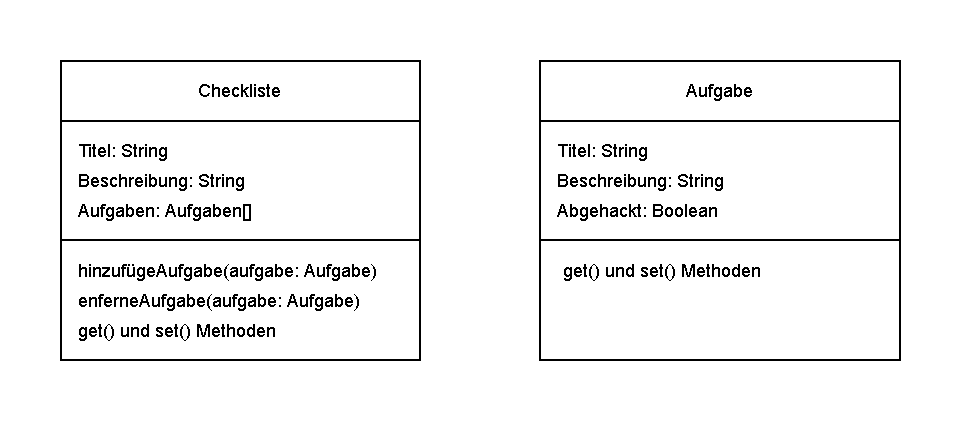
\includegraphics{Bilder/KlassenDiagramm.pdf} 
	\caption{Klassen-Diagramm zu den Grundlegenden Klassen Checkliste und Aufgabe}
	\label{fig:KlassenDiagramm}
\end{figure}

\section{Risikobehandlung}\label{sec:risiko}

Zum Schluss des Planungskapitel und somit der ursprünglichen Projektdefinition wird das Thema Risikobehandlung behandelt.
Die Risikobehandlung dient dem einschätzen und eingrenzen von Risiken. Dabei werden mögliche Risiken erfasst und beschrieben. Dazu zählen das Risiko, eine Beschreibung zu dem Risiko, eine geschätzte Wahrscheinlichkeit zu der das Risiko eintritt und eine Alternative mit welcher im Falle des Auftretens die Auswirkungen aufgefangen oder abgemildert werden soll. In \autoref{tabelle:Risko} wird die Risikobehandlung aus der Projektdefinition dargestellt.
\begin{table}[h]
	\centering
	\caption{Risikobehandlung}
	\begin{tabularx}{\textwidth}{|X|X|>{\centering\arraybackslash}X|X|}
		\toprule
		Risiko  & Beschreibung & Wahrscheinlichkeit & Alternative\\ \midrule 
		Verspäteter Projektstart  & Die Bearbeitung des Studienarbeitsprojekt wird verspätet angefangen & 80\%  & Verlorene Zeit wird zu einem späteren Zeitpunkt durch längere Arbeitstage und Wochenendschichten aufgeholt \\ \midrule
		Umfang nicht eingehalten & Aufgrund von Zeit oder Wissensmangel nicht alle Anwendungsfälle in der App implementiert & 20\% & Leistungsumfang im Bereich des möglichen verringern \\ \midrule
		Krankheit & Verminderter Fortschritt aufgrund von Krankheit & 20\% & Krankheit so gut wie möglich vermeiden, verlorene Zeit später aufholen \\ \midrule
		Vernachlässigte Dokumentation & Nicht alle Ideen und konkret geplante Umsetzungen vor der Implementierung dokumentiert & 50\% & Wenn möglich Dokumentation nachholen (Bsp. Diagramme) \\
		\bottomrule
	\end{tabularx}
	\label{tabelle:Risko}
\end{table}

Wie in \autoref{tabelle:Risko} zu sehen ist hält sich die Anzahl an Risiken in grenzen. Dies ist darauf zurückzuführen das nur eine Person und kein Team an dem Projekt arbeitet. Dadurch können keine Kommunikationsprobleme auftreten. Ausfälle einzelner Personen und somit Nichterfüllung derer Aufgabenteile reflektieren hier das ganze Projekt und könnten somit alle mit den vier genannten Risiken abgedeckt werden.\\
Da es sich bei den in der Tabelle aufgeführten Risiken um die aus der Projektdefinition handelt werden eventuelle Eintritte und Erweiterungen im folgenden erläutert.\\
Das Risiko des verspäteten Projektstart ist wie anfangs korrekt eingeschätzt wurde eingetreten. Damit hat sich die Eintrittwahrscheinlichkeit von 80\% bestätigt. Das Eintreten des Risiko ist auf eine schlechte Angewohnheit des Verantwortlichen zurückzuführen. Die Alternative zu diesem Risiko befindet sich in Ausübung und wird mit Ende der Ausarbeitung der Studienarbeit als erfolgreich angesehen.\\
Das zweit genannte Risiko konnte nach Projektdefinitionsstand erfolgreich verhindert werden. Das Risiko wird jedoch hiermit um \glqq Erweiterungsumfang nicht eingehalten\grqq erweitert, da nach Rücksprache mit dem Betreuer sind Ideen für weitere Anwendungsfälle aufgetreten. Die Wahrscheinlichkeit für dieses angepasste Risiko wird somit im Nachhinein auf 60\% angehoben. Die Alternative für Eintritt des Risiko wird beibehalten und vermutlich Anwendung für den Großteil der Ideen finden.\\
Die vernachlässigte Dokumentation ist ebenfalls in kleinerem Rahmen eingetreten. Die Studienarbeit selbst gilt als Hauptaspekt der Dokumentation und wird sicher fertiggestellt. Der eingetretene Bereich bezieht sich auf das erstellen von \ac{UML}-Diagrammen. Hier tritt ebenfalls die Alternative in Kraft und Diagramme werden nach Bedarf erstellt.\\
Das Risiko Krankheit konnte zu 100\% vermieden werden.\\
In Folge des \autoref{chpt:durchfuerung} \nameref{chpt:durchfuerung} werden unerwartete Probleme aufgeführt, welche Aufgrund des unerwarteten Eintritts keine Berücksichtigung in der Risikobehandlung gefunden haben. Diese werden im \autoref{sec:problem} \nameref{sec:problem} behandelt.\\

Mit Abschluss der Risikobehandlung gilt das \autoref{chpt:planung} \nameref{chpt:planung} als abgeschlossen. In diesem Kapitel wurden die Projektdefinition welche zu Beginn des Projekts stattgefunden hat behandelt. Es wurde die konkrete Projektdefinition ausgeführt und mithilfe der Rahmenbedingungen und des Umfang eingegrenzt und konkretisiert. Als Abschluss wurde auf die Risikobehandlung eingegangen und eventuelle Eintritte und Änderungen erläutert.
\chapter{Durchführung}\label{chpt:durchfuerung}

Dieses Kapitel beschreibt die Durchführung des Projekts. Explizit wird hier der Beginn und Verlauf der Entwicklung der \glqq Leave The House\grqq-App behandelt. Zu Beginn wird der Start der Projektdurchführung, gefolgt von der eigentlichen Entwicklung beschrieben. Im Anschluss daran wird das Testen der Applikation behandelt. Zum Schluss dieses Kapitels werden in der Problembehandlung alle in den Anderen Abschnitten aufgetretenen Probleme ausführlich behandelt.

\section{Projektdurchführung}\label{sec:projektdurchfuerung}

Die Projektdurchführung behandelt den Start der eigentlichen Arbeit des Projekts. Wie bereits in \autoref{chpt:planung} beschrieben ist das Risiko des verspäteten Projektstarts eingetreten. Dies führte dazu, dass die Arbeit an dem Projekt nicht wie geplant am 01.01.2020 gestartet wurde. Der Projektstart begann stattdessen im März 2021. Durch die in der \nameref{sec:risiko} festgelegte Alternative hatte der verspätete Start keine, abgesehen der aus der Alternative resultierenden, Auswirkungen auf die Durchführung.\\
Die Bearbeitung des Projekts begann im März 2021 und endete mit Erreichung des geplanten Umfang Mitte April 2021. Durch die bereits genannte Erweiterung des Umfang nach Rücksprache mit dem Betreuer wird der endgültige Projektabschluss auf das Abgabedatum der Studienarbeit, den 17.05.2021, verlegt. Das Ende der Bearbeitung des zuvor geplanten Umfang wird weiterhin als Mitte April festgehalten. In der Verlängerten Bearbeitungszeit wird versucht die weiteren Ideen für den Umfang des Betreuer zu implementieren, da in dieser Zeit auch die Studienarbeit geschrieben werden muss kann eine vollständige Dokumentation dieser in der Studienarbeit nicht gewährleistet werden.

\section{Entwicklung}\label{sec:entwicklung}
In diesem Abschnitt wird der vollständige Verlauf der Entwicklung behandelt. Von der Erstellung des Projekts bis hin zum ersten fertigen Zustand der App. Die während der Entwicklung aufgetretenen Probleme werden hier genannt, jedoch erst im \autoref{sec:problem} \nameref{sec:problem} ausführlich behandelt. Das erstellen der im Umfang festgelegten Tests wird ebenfalls in einem anderen Abschnitt (\ref{sec:tests} \nameref{sec:tests}) behandelt.

\subsection{Projekterstellung}\label{subsec:projekterstellung}
Zu Beginn der Arbeit an einem Projekt muss zuerst das Projekt erstellt werden. Dies hängt damit zusammen, dass \acp{IDE} in der Regel Projekte als oberste Ordnerstruktur nutzen. Alle Dateien innerhalb des Projektordners können somit diesem Projekt zugeordnet werden.\\
Die Entwicklung der App begann ebenfalls mit der Erstellung eines neuen Projekts in Android Studio. Dabei wird \glqq New $\rightarrow$ New Project\grqq{} in der File Dropdown-Liste ausgewählt. Da Android nicht nur als Betriebssystem für Smartphones und Tablets sondern auch für Smartwatches oder in Autos und TVs verwendet wird muss als erster Schritt angegeben werden für welche Endplattform man eine Anwendung entwickeln möchte. In diesem Schritt kann auch direkt eine Projektvorlage ausgewählt werden. Aufgrund von geringer Erfahrung in der App-Entwicklung wurde für dieses Projekt die Vorlage \glqq Basic Activity\grqq (Basis Aktivität) anstatt einer \glqq Empty Activity\grqq (Leere Aktivität) als Grundlage für das Projekt gewählt. Im Gegensatz zu einer leeren Aktivität Vorlage beinhaltet die Basic Activity bereits ein Einstellungsmenü in der Werkzeugleiste am oberen Bildschirmrand, einem Knopf in der unteren Rechten Bildschirmecke und einen Knopf in der Mitte des Bildschirms, der einen Anzeigenwechsel bewirkt. Diese bereits vorhandenen Elemente und Funktionen erleichtern den Einstieg in die Entwicklung, da der Entwickler sich den Code dieser ansehen und somit leichter die Funktionsweise und Aufbau von Android-Apps verstehen kann. Hilfreich hierbei ist der in der Android Studio \ac{IDE} eingebaute Emulator. Mit dem Emulator können virtuelle Android Geräte erstellt werden, um die App zu testen. Dabei kann die Android Version, so wie das Gerät ausgewählt werden. Der Emulator ist direkt zu Projektstart der Punkt an dem das erste Problem auftrat. Nach erstellen des Projekts kann man die gewählte Vorlage direkt über den Emulator testen. Dafür muss im AVD Manager ein neues Gerät erstellt werden, welches zum testen genutzt werden soll. Bis hierhin lief alles reibungslos. Beim ausführen der App kam jedoch dann das Problem zum Vorschein, der Emulator konnte nicht gestartet werden.
Es blieben nun nur zwei Möglichkeiten das Problem zu beheben, welche im \autoref{sec:problem} \nameref{sec:problem} behandelt werden. Nach wählen der Vorlage müssen noch weitere Informationen bei der Projekterstellung angegeben werden.
Einerseits muss der Name des Projekts angegeben werden, hier wurde der Name der Endgültigen App \glqq Leave The House\grqq{} eingegeben. Andererseits müssen grundlegende Entscheidung für die Entwicklung der App gefällt werden. Neben dem Namen muss noch die Programmiersprache und die minimal kompatible Anrdoid-Version gewählt werden. Android Apps können in zwei verschiedenen Sprachen geschrieben werden. Java und Kotlin. Für dieses Projekt wurde Kotlin als Programmiersprache für die App ausgewählt. Kotlin ist in der Android Entwicklung weit verbreitet und bietet eine Interoperabilität für Java. Somit kann während der App-Entwicklung auch auf Java zurückgegriffen werden, falls dies nötig sein sollte. Kotlin bietet im Gegensatz zu Java weitere Features wie null-Absicherung zurm Schutz vor NullPointer-Exceptions oder direkte View.Bindung.\footcite{Kotlin.2020} Als minimale Android-Version wurde die \ac{API} (Programmierschnittstelle) 23 festgelegt. Diese entspricht der Android Version 6.0 Marshmello und wird laut Android Studio zum aktuellen Zeitpunkt von 84.9\% der Geräte unterstützt. Nach diesen Angaben wurde die Erstellung des Projekts in Android Studi erfolgreich abgeschlossen. An diesem Punkt (nach Behebung des Problems) könnte mit der Entwicklung begonnen werden, doch ein wichtiges weit verbreitetes und empfohlenes Mittel kann noch zum Projekt hinzugefügt werden. Die Versionsverwaltung.\\
Mithilfe von Versionsverwaltung können Änderungen an Dateien erfasst und verwaltet werden. Ein übliches Versionsverwaltungssystem ist der kostenlose Dienst GitHub. In GitHub können Nutzer für Projekte sogenannte \glqq Repository\grqq, zu Deutsch Verwaltungsorte, anlegen. Innerhalb eines Repository werden die Projektdateien verwaltet. GitHub erfasst jede Änderung an einer Datei und kann diese dem Nutzer anzeigen. Mithilfe eines commit können die Änderungen dann als neue Version im Repository abgelegt werden. Dies erlaubt es mehreren Nutzern an der gleichen Datei zu arbeiten ohne sich ständig in die Quere zu kommen. Außerdem erlaubt es dem Nutzer immer wieder auf stabile Versionen zurückzugreifen falls die aktuellen Änderungen nicht zum gewollten Ergebnis geführt haben. Im Zuge dieses Projektes wurde auf GitHub ein neues Repository angelegt, welches als Versionsverwaltung für die App genutzt wird. Damit können beispielsweise erfolgreiche Implementierungen eines Anwendungsfalls mithilfe eines commits in GitHub gesichert werden.\\
Mit der Erstellung des GitHub Repository und Verknüpfung des Android Studio Projekts damit ist die Projekterstellung abgeschlossen. Alle Vorbereitungen sind somit getroffen worden um eine Erfolgreiche Entwicklung zu gewährleisten.


\subsection{Erstellen der Checkliste}\label{subsec:erstelleChecklisten}

Nach der erfolgreichen Projekterstellung begann die Arbeit an dem Projekt mit der Realisierung des ersten Anwendungsfall, dem erstellen einer Checkliste. Dafür wurde die Klasse Checkliste angelegt, diese wird in \autoref{code:checkliste} gezeigt. Die Klasse besteht aus einem initialen Konstruktor, welcher den Titel und die Beschreibung, sowie einem zweiten Konstruktor der neben Titel und Beschreibung noch eine Liste von Aufgaben entgegennimmt. Zudem enthält die Klasse, wie in \autoref{sec:umfang} beschrieben, die Methoden um ein Element der Aufgaben Liste hinzuzufügen und um ein Element aus der Liste zu entfernen. Die ebenfalls beschrieben get() und set() Methoden sind in dieser Klasse nicht vorhanden, da Kotlin diese Methoden standardmäßig durch Zugriff auf die Variable zur Verfügung stellt. Um also auf den Titel einer Checkliste zuzugreifen genügt $checklist.title$ anstelle von $checklist.getTitle()$. Nachdem das Modell zum halten der Checkliste, die Checkliste-Klasse erstellt wurde muss nun die Funktion implementiert werden ein Checklisten Objekt zu erstellen und auf dem Bildschirm anzuzeigen.
\\
\lstinputlisting[
label=code:checkliste,    % Label; genutzt für Referenzen auf dieses Code-Beispiel
caption=Checkliste Klasse,
captionpos=b,               % Position, an der die Caption angezeigt wird t(op) oder b(ottom)
style=EigenerKotlinStyle,     % Eigener Style der vor dem Dokument festgelegt wurde
firstline=1,                % Zeilennummer im Dokument welche als erste angezeigt wird
lastline=14                 % Letzte Zeile welche ins LaTeX Dokument übernommen wird
]{Quellcode/Checkliste.kt}

Bevor diese Funktion jedoch implementiert werden kann muss der Ablauf dafür festgelegt werden. Der Nutzer soll auf den in der rechten unteren Bildschirmecke befindlichen Knopf drücken um eine neue Ansicht zu öffnen. Diese zeigt Eingabefelder für den Titel und die Beschreibung in denen der Benutzer diese Angaben tätigt, welche dann für den Konstruktor der Checklisten Klasse genutzt werden. Über einen Knopf an der gleichen Position wie der vorherige wird die Eingabe bestätigt und die Checkliste mit den Eingegeben Werten erstellt. Die erstellte Checkliste soll dann als Element einer Liste auf dem Bildschirm dargestellt werden. Anhand dieses Ablaufs wurde dann die Implementation dieser Funktion und Anwendungsfall begonnen. \autoref{fig:mainActivity} und \autoref{fig:createChecklist} zeigen die Layouts zu dem beschrieben Ablauf.\\
Android besteht Grundlegend aus Aktivitäten. Die Grundaktivität ist die sogenannte \glqq Main Activity\grqq. Diese bildet den Einstiegspunkt in die App und wird beim öffnen der App angezeigt. Eine Aktivität besteht meistens aus einer \grqq Controller-\grqq{} und einer Layout Datei. In der Layout-Datei wird definiert was auf dem Bildschirm angezeigt wird wenn die Aktivität ausgeführt wird. Dabei handelt es sich um eine XML-Datei in der Elemente wie Knöpfe, Text oder weitere mithilfe eines Layouts angeordnet werden können. Die Controller-Datei spiegelt dagegen die funktionale Ebene der Aktivität wieder. In ihr werden Funktionen ausgeführt und der Aktivitäts-Lebenszyklus behandelt. Eine Aktivität hat einen Lebenszyklus der aus verschiedenen Zuständen besteht. Der erste Zustand der ausgeführt wird ist \glqq onCreate()\grqq. In dieser Methode wird angegeben welches Layout dem Nutzer angezeigt werden soll. Diese Methode wird in der Regel immer überschrieben, um mittels setContentView() das Layout anzugeben. \autoref{code:onCreate} zeigt die onCreate-Methode der Aktivität CreateChecklist. Hier wird wie angegeben die onCreate-Methode überschrieben und über setContentView das zugehörige Layout zur Darstellung auf dem Bildschirm angegeben. Zudem wird über die seSupportActionBar-Methode die im Layout definierte Werkzeugleiste als SupportActionBar festgelegt. Damit wird der Aktivität ermöglicht die Interaktion mit eventuell in der Werkzeugleiste vorhanden Knöpfen zu erfassen und entsprechende Funktionen auszuführen. In der weiteren Beschreibung zur Implementierung des Anwendungsfall zum erstellen einer Aktivität wird weiter auf das Codebeispiel eingegangen. Die weiteren Zustände des Lebenszyklus sind onStart() (Startet die Aktivität und macht sie sichtbar und ermöglicht Interaktivität), onResume() (Wird ausgeführt wenn die Aktivität wieder Interagierbar wird), onPause() (Dieser Zustand tritt auf wenn die Aktiviät den Fokus verliert und ist oft ein Indikator dass die Aktivität verlassen wird), onStop() (Die Aktivität ist nicht länger sichtbar für den Nutzer), onRestart(Wechsel von onStop() in onStart()) und onDestroy() (Zerstört die Aktivität und endet den Lebenszyklus).\footcite{Aktivitäten.2021} Die Grundlegende Funktionsweise von Aktivitäten sollte nun verstanden worden sein.\\
Um den Anwendungsfall eine Checkliste erstellen zu realisieren wird zunächst eine neue Aktivität erstellt. Dazu wird über File $\rightarrow$ New $\rightarrow$ Activity $\rightarrow$ Empty Activity eine neue Aktivität angelegt. Hierbei muss der Name der Aktivität und des Layout angegeben werden. Der Name des Layout wird von Android Studio passend zu der Eingabe im Aktivitätsnamen-Feld angepasst. Auch hier kann die Programmiersprache gewählt werden. Das lässt sich auf die Interoperabilität zurückführen, da damit auch eine Java-Aktivität in einer Kotlin Anwendung ausgeführt werden kann.\\
In der onCreate-Methode wird wie bereits verdeutlicht das Layout für die Aktivität festgelegt. Das für die CreateActivity erstellte Layout kann in \autoref{fig:createChecklist} eingesehen werden. Es stellt jeweils ein Label sowie ein Eingabefeld für den Titel und die Beschreibung dar. Zusätzlich befindet sich in der unteren rechten Ecke ein Knopf über den die Checkliste mit den Eingaben aus den Eingabefeldern hinzugefügt werden soll.\\
Um dieses Layout auf dem Bildschirm zu sehen muss zunächst die dazugehörige Aktivität gestartet werden. Wie bereits erläutert wird die App mit der MainActivity gestartet, welche als Einstiegspunkt für die Anwendung dient. Das Layout der MainActivity kann in \autoref{fig:mainActivity} angesehen werden. Dieses Layout besteht aus einer Werkzeugleiste, der bereits im Ablauf für den Anwendungsfall beschriebene Liste in Form einer RecyclerView zum Anzeigen der Checklisten und dem aus der Vorlage übernommenen und angepassten Knopf. Mit diesem Knopf soll der Anwendungsfall und die createChecklist Aktivität gestartet werden. Um dem Knopf die Funktionalität dafür zu geben wird er zunächst über die findViewById-Methode der Knopf mithilfe der ID gefunden, um so mit ihm innerhalb dieser Klasse interagieren zu können. Für die Interaktion wird der Knopf mit einem onClickListener versehen. Dieser führt die darin geschriebene Funktion aus sobald der Nutzer den Knopf betätigt. In diesem Fall soll die CreateChecklist Aktivität gestartet werden. Dazu wird ein Intent deklariert. Ein Intent ist ein Nachrichten-Objekt das genutzt wird um Aktionen von einer anderen Anwendungskomponente anzufragen. Das starten einer Aktivität stellt einen der drei fundamentalen Anwendungsfälle des Intent Objekts dar.\footcite{Intents.2021} Der Codeausschnitt \autoref{code:onCreateInMain} zeigt die Deklaration des Intent un der darauffolgende Aufruf zum starten der CreateChecklist Aktivität im onClickListener des Knopf. Bei der Initialisierung des Intent muss die jeweilig zu startende Aktivität als Parameter übergeben werden. Diese wird im Anschluss mit dem Befehl startActivity() oder in diesem Fall startActivityForResult() durch Übergabe des Intent in den Befehl gestartet. Zusätzlich wird beim Starten der Aktivität ein weiterer Parameter übergeben. Dieser stellt einen requestCode dar mit dessen Hilfe Ergebnisse von Aktivitäten unterschieden werden können. Das ermöglicht den korrekten Umgang mit den im Ergebnis potentiell übergebenen Daten.
\\
\lstinputlisting[
label=code:onCreateInMain,    % Label; genutzt für Referenzen auf dieses Code-Beispiel
caption=Start der CreateChecklist Aktivität,
captionpos=b,               % Position, an der die Caption angezeigt wird t(op) oder b(ottom)
style=EigenerKotlinStyle,     % Eigener Style der vor dem Dokument festgelegt wurde
firstline=1,                % Zeilennummer im Dokument welche als erste angezeigt wird
lastline=4                 % Letzte Zeile welche ins LaTeX Dokument übernommen wird
]{Quellcode/startOnCreateInMain.kt}

Nachdem die Aktivität gestartet wurde wird, wie mit dem Aktivitäts-Lebenszyklus beschreiben die onCreate-Methode der CreateChecklist Aktivität ausgeführt. Wie in \autoref{code:onCreate} zu sehen wird dort ebenfalls der Knopf mit einem onClickListener versehen. Dieser beendet im Gegensatz zum anderen die Aktivität anstatt eine neue MainActivity zu starten. Allerdings wird ebenfalls ein Intent erstellt. Mithilfe des Intent werden die Nutzereingaben der MainActivity als Ergebnis der createActivity Aktivität übergeben. Um die Nutzereingaben zu lesen werden die Textfelder, wie die Knöpfe zuvor, mithilfe der ID gefunden un der deren Text-Attribut ausgelesen. Die putExtra-Methode des Intent erlaubt es über einen Intent zusätzliche Daten zu übergeben. Dazu muss in dieser Methode ein Schlüssel-Wert Paar erstellt werden. Nachdem die Nutzereingaben dem Intent beigefügt wurden wird dieser in der setResult-Methode zusammen mit einem RequestCode übergeben. Der RequestCode spiegelt hier den gleichen wieder der auch zum starten der Aktivität übergeben wurde. Die zwei darauffolgenden Methodenaufrufe dienen dem Beenden der Aktivität.
Das Ergebnis wird durch die onActivityResult-Methode weiter verarbeitet, welche in \autoref{code:onActivityResult} teilweise einsehbar ist. Diese wird, wie die onCreate-Methode, überschrieben um eigenen Code ausführen zu können. Die Methode bekommt als Parameter einen RequestCode, einen resultCode und einen Intent als Datenhalter übergeben. Hier wird der Nutzen des requestCode deutlich. Er wird als Schlüsselvariable für den Switch genutzt, um Ergebnisse aus unterschiedlichen Aktivitäten unterscheiden zu können. Für den Aktuellen Stand von nur einer Aktivität wäre der Switch nicht notwendig, da im weiteren verlauf der Entwicklung weitere hinzukommen wurde er bereits von Anfang an implementiert. Der resultCode stellt den Status des Ergebnis der Aktivität dar und könnte beispielsweise Result.OK lauten. Dieser findet hier allerdings keine Verwendung da die Ergebnisüberprüfung über ein Extra des Intent behandelt wird. Bei dem Intent handelt es sich um den in der setResult-Methode übergebenen Intent. Zu Beginn der Bearbeitung der vom Intent übergebenen Daten wird über das \glqq successful\grqq{}-Extra geprüft ob das übergeben der Daten erfolgreich war. Im Anschluss wird ein neues Checklisten-Objekt erstellt. Dieses erhält als Parameter die vom Nutzer in der CreateChecklist Aktivität eingegebenen Titel und Beschreibung. Im Anschluss daran wird überprüft ob der Eingegebene Titel ein Duplikat ist. Falls dem so ist wird die neue Checkliste nicht der Liste von Checklisten zugefügt, welche als Datenhalter in der Main-Aktivität dient, und eine Fehlermeldung auf dem Bildschirm angezeigt. Falls nicht wird die neue Checkliste der Liste hinzugefügt und infolgedessen auf dem Bildschirm angezeigt.
\\
\lstinputlisting[
label=code:onCreate,    % Label; genutzt für Referenzen auf dieses Code-Beispiel
caption=onCreate Methode der CreateChecklist Aktivität,
captionpos=b,               % Position, an der die Caption angezeigt wird t(op) oder b(ottom)
style=EigenerKotlinStyle,     % Eigener Style der vor dem Dokument festgelegt wurde
firstline=1,                % Zeilennummer im Dokument welche als erste angezeigt wird
lastline=21                 % Letzte Zeile welche ins LaTeX Dokument übernommen wird
]{Quellcode/onCreate.kt}

\lstinputlisting[
label=code:onActivityResult,    % Label; genutzt für Referenzen auf dieses Code-Beispiel
caption=onActivityResult Methode der Main Aktivität,
captionpos=b,               % Position, an der die Caption angezeigt wird t(op) oder b(ottom)
style=EigenerKotlinStyle,     % Eigener Style der vor dem Dokument festgelegt wurde
firstline=1,                % Zeilennummer im Dokument welche als erste angezeigt wird
lastline=25                 % Letzte Zeile welche ins LaTeX Dokument übernommen wird
]{Quellcode/onActivityResult.kt}

Die Checklisten sollen in Form einer Liste auf dem Bildschirm dargestellt werden. Dazu wird wie im Layout der MainActivity beschrieben eine RecyclerView genutzt. Im Vergleich zu einer herkömmlichen ListView ist die RecyclerView eine modernere, flexiblere und performantere Alternative. Im Gegensatz zu Knöpfen und Textfeldern kann die RecyclerView nicht einfach mithilfe der ID gefunden und beispielsweise der Text gesetzt werden. Um Einträge in der RecyclerView anzuzeigen wird ein Adapter benötigt. Das ist Notwendig da jedes Item in der Liste als separate View behandelt wird und gesondert dargestellt werden muss. Um die Checklisten in der RecyclerView darstellen zu können wurde der ChecklistRecyclerViewAdapter als Klasse angelegt. Dieser erhält als Parameter die Liste von Checklisten aus der MainActivity, da diese die Informationen zu den Items hält die Dargestellt werden sollen. Zusätzlich wird innerhalb dieser Klasse eine weitere Klasse erstellt. Diese Klasse ist ein ViewHolder und heißt ChecklistViewHolder. Jedes Item in der RecyclerView wird durch eine Instanz dieses ViewHolder definiert. Für jeden Eintrag in der Liste wird vom Adapter ein ViewHolder erstellt und im Anschluss daran die Daten daran gebunden. \autoref{code:ViewHolder} zeigt die Methoden onCreateViewHolder und onBindViewHolder des ViewHolder. Ähnlich wie bei den Aktivitäten wird in der onCreate-Methode das Layout festgelegt. Bei dem Layout handelt es sich um ein speziell für die Liste erstelltes Layout, welches einen Eintrag der Liste repräsentiert. In \autoref{fig:mainActivity} können drei dieser Listenitems gesehen werden. Diese bestehen aus einem Textfeld für den Titel der Checkliste und einem weiteren, etwas nach rechts gerücktem, mit kleinerer und grauer Textfont versehenen Textfeld für die Beschreibung. Die onBindViewHolder-Methode setzt den Text dieser Textfelder, sodass die richtigen Daten angezeigt werden.
In der MainActivity wird um die Daten darzustellen die RecyclerView anhand der ID gefunden und eine Instanz des Adapter erstellt. Dabei wird die Liste der Checkliste als darzustellende Items übergeben. Damit frisch erstellte Checklisten in der Liste angezeigt werden wurde die onActivityResult-Methode um dem Funktionsaufruf 
$checklistRecyclerView.adapter?.notifyDataSetChanged()$ erweitert. Dieser teilt dem Adapter mit, dass sich die Daten verändert haben und veranlasst so ein neu laden der Liste.\\
\\
\lstinputlisting[
label=code:ViewHolder,    % Label; genutzt für Referenzen auf dieses Code-Beispiel
caption=ViewHolder Methoden des ChecklistRecyclerViewAdapter,
captionpos=b,               % Position, an der die Caption angezeigt wird t(op) oder b(ottom)
style=EigenerKotlinStyle,     % Eigener Style der vor dem Dokument festgelegt wurde
firstline=1,                % Zeilennummer im Dokument welche als erste angezeigt wird
lastline=12                 % Letzte Zeile welche ins LaTeX Dokument übernommen wird
]{Quellcode/ViewHolder.kt}

\begin{figure}[h]
	\centering
	\begin{minipage}{0.45\linewidth}
		\centering
		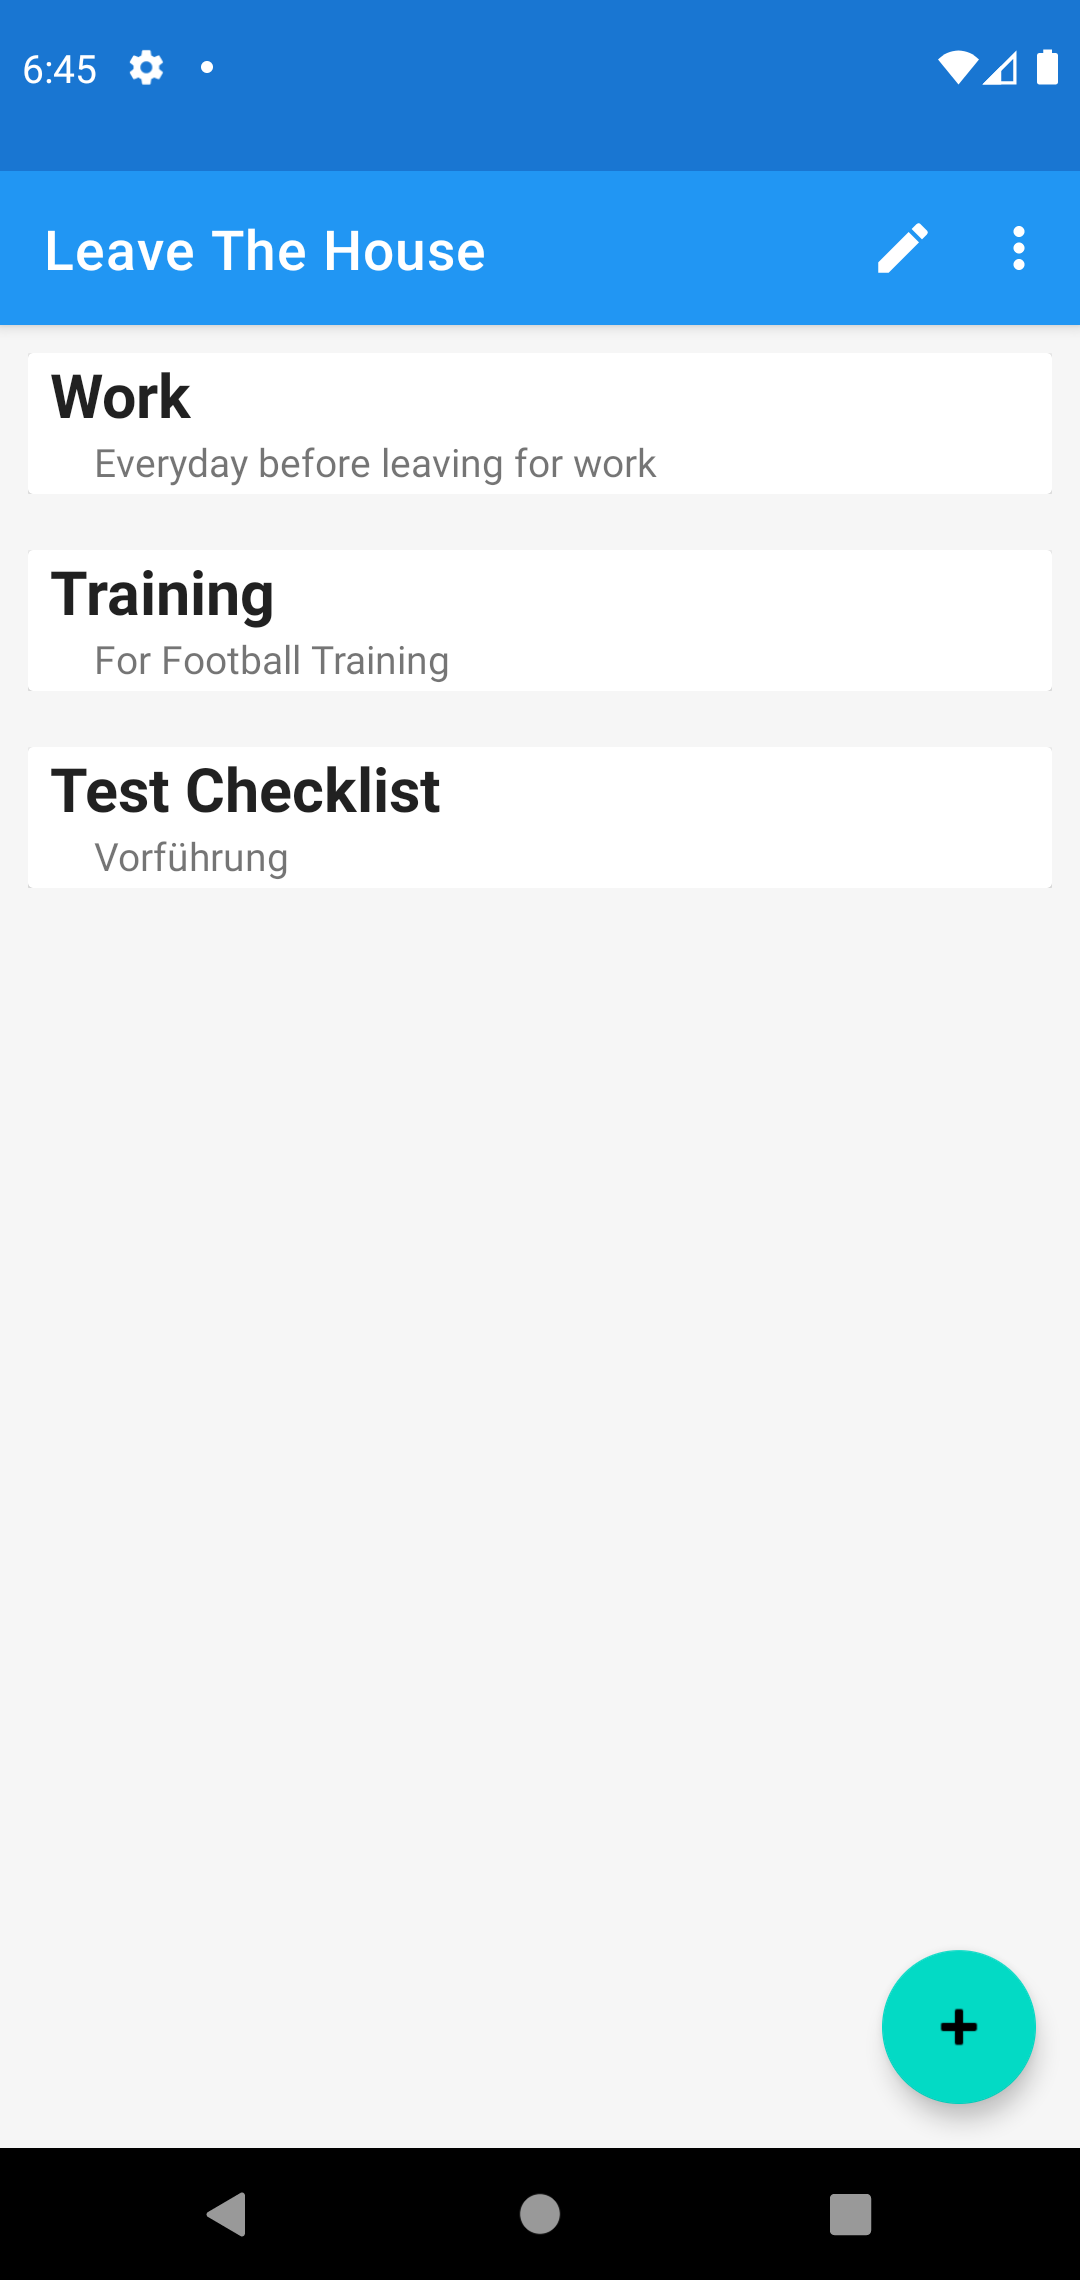
\includegraphics[width=.9\linewidth]{Bilder/MainActivity.png}
		\caption{MainActivity Ansicht}
		\label{fig:mainActivity}
	\end{minipage}
	\hfill
	\begin{minipage}{0.45\linewidth}
		\centering
		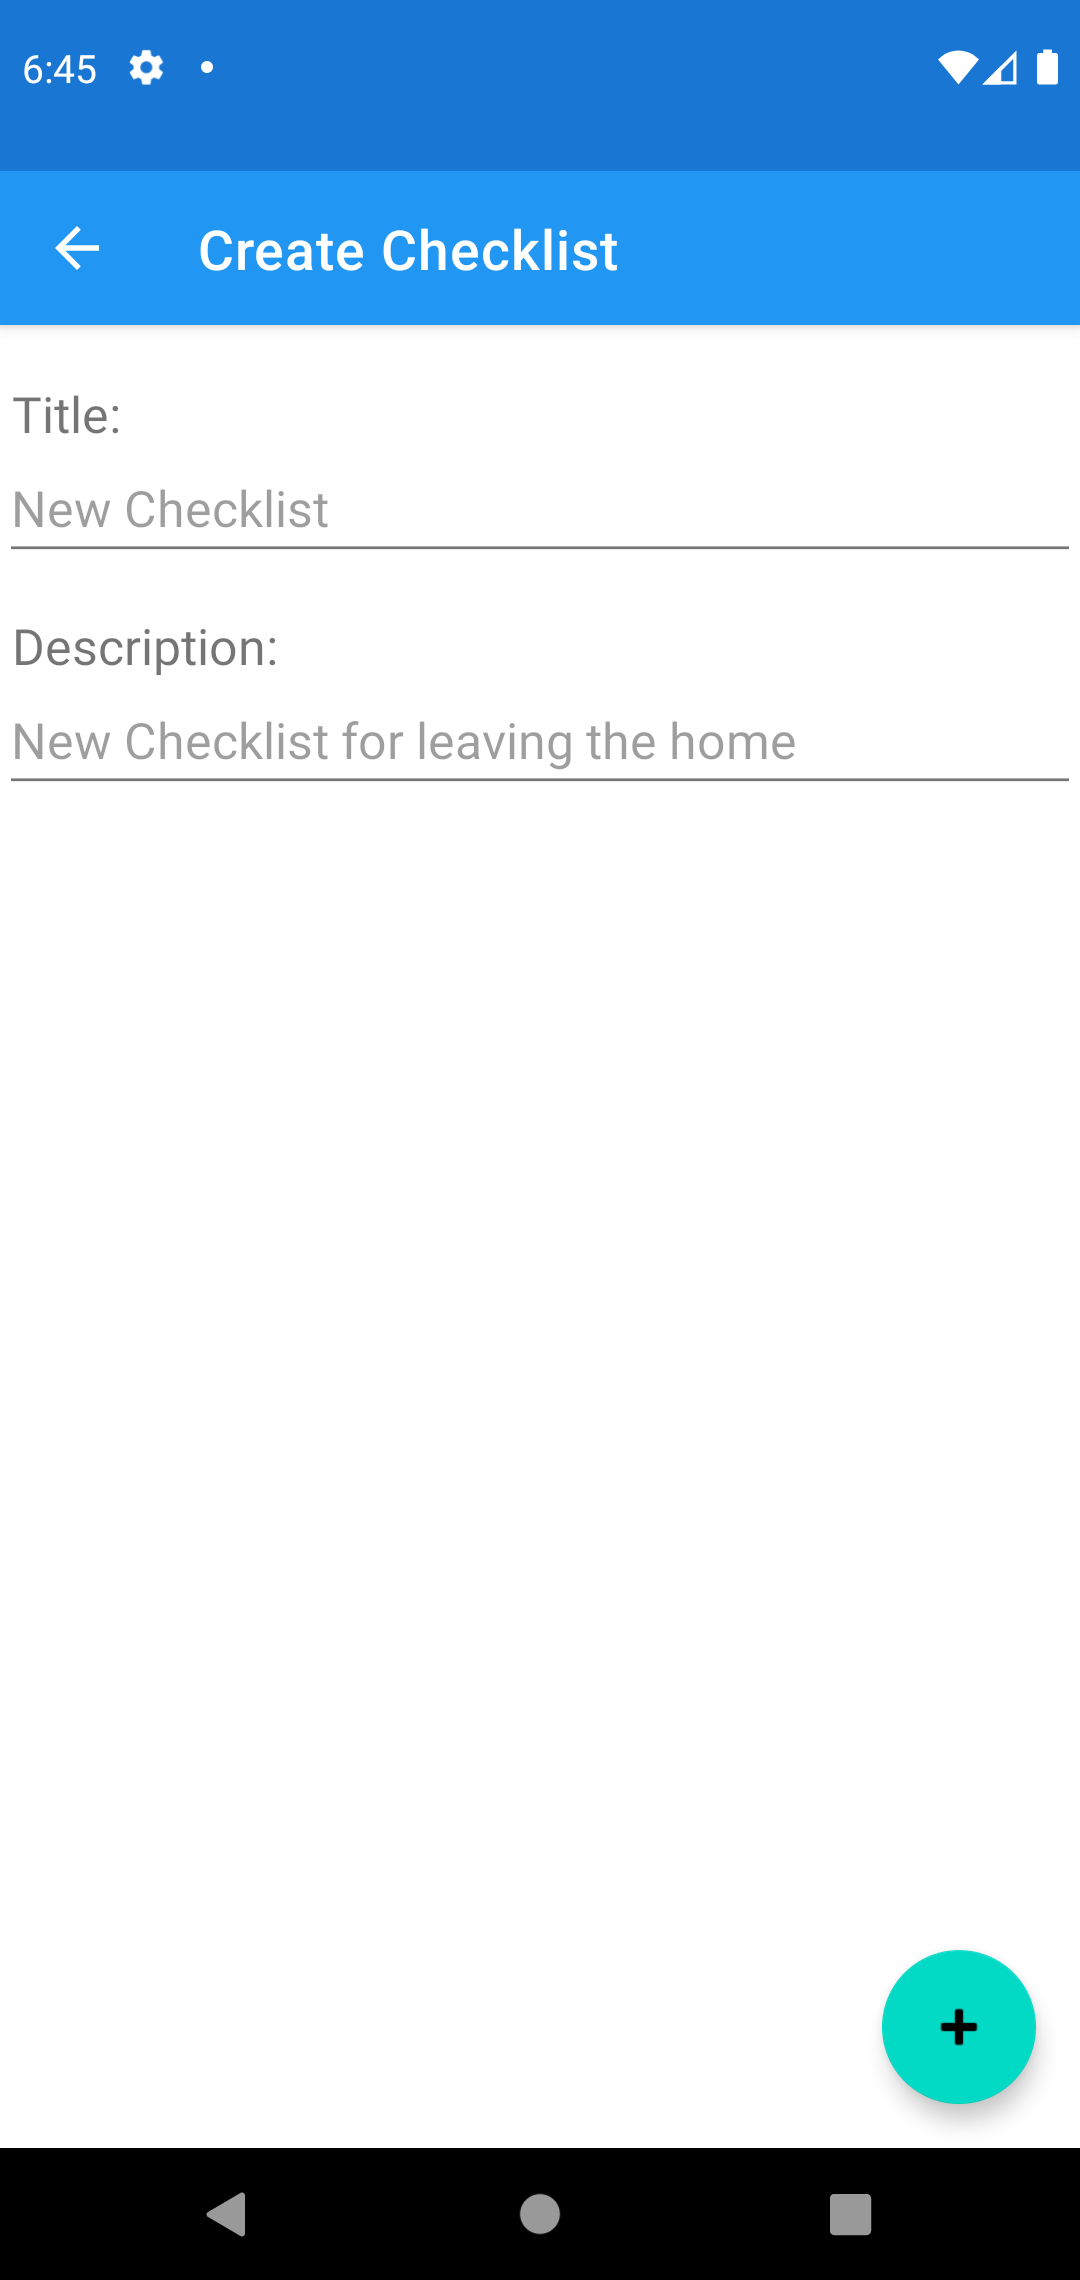
\includegraphics[width=.9\linewidth]{Bilder/CreateChecklist.png}
		\caption{CreateChecklist Ansicht}
		\label{fig:createChecklist}
	\end{minipage}
\end{figure}

Mit dem darstellen der erstellten Checkliste kann der erste Anwendungsfall, das erstellen einer Checkliste, nahezu als erfolgreich implementiert angesehen werden. Es ist dem Nutzer möglich über den Knopf die CreateChecklist Aktivität zu starten und seine Eingaben für Titel und Beschreibung zu tätigen. Durch bestätigen der Eingaben wird das neue Checklisten Objekt erstellt und dynamisch in der RecyclerView-Liste eingefügt und dargestellt. Der letzte fehlende Schritt ist das speichern und laden von erstellten Checklisten. Dieser Schritt wird in \autoref{subsec:speichereCheckliste} erläutert.

\subsection{Speichern von Checklisten}\label{subsec:speichereCheckliste}

Nachdem es dem Nutzer möglich ist Checklisten zu erstellen ist der nächste Schritt die erstellte Checkliste zu speichern und beim öffnen der App die gespeicherten Checklisten wieder zu laden und in der RecyclerView anzuzeigen.\\
Die erste Überlegung war hierfür ein Backend zu entwickeln, welches die Daten in einer Datenbank speichert und über eine \ac{API} ansprechbar ist. Voraussetzung für diese Herangehensweise wäre ein Nutzer-System. Jeder Nutzer müsste einen Account erstellen und diesen mit einem Passwort absichern. Ohne das könnten die gespeicherten Checklisten nicht dem richtigen Benutzer zugeordnet werden. Im verlauf der Entwicklung wurde sich gegen diese Herangehensweise entschieden und stattdessen das Speichern der Daten in einer Datei auf dem gerät gewählt. Grund dafür sind teilweise persönliche Präferenzen und Abwägung an den Vorteilen, die eine solche Lösung mit sich bringen würde. Auf der einen Seite würde es dem Nutzer ermöglichen Speicher auf dem Endgerät zu sparen. Auf der anderen Seite jedoch müsste ein Nutzer sich einen Account erstellen, bei dem er eine valide E-Mail Adresse, eventuell einen Nutzernamen und ein Passwort festlegen nur um Checklisten erstellen zu können. Zusätzlich müsste die Anwendung eine Internetverbindung haben und der Nutzer somit der App diesen Zugriff auf seinem gerät erlauben. Diese Punkte spiegeln auch die persönlichen Ablehnungen für diese Herangehensweise wieder, da ich dem erstellen von Accounts für skeptisch gegenüberstehe und dabei auch schon schlechte Erfahrungen mit Veröffentlichung von E-Mail Adressen nach Angriffen auf die Server gesammelt habe. Zudem sollte man für das erstellen und speichern einer Checkliste keine Internetverbindung brauchen, wobei dieser Punkt in der heutigen zeit zu vernachlässigen ist da jedes Endgerät, zumindest Zuhause per WLAN, eine Internetverbindung hat. Für diese App wurde sich jedoch für das lokale Speichern der Daten in einer Datei entschieden. Android unterstützt diese Herangehensweise durch das interne Datei System. Dies ermöglicht es Dateien Lokal auf dem Gerät persistent zu speichern. Als Format wurde hierfür die \ac{JSON} gewählt. Bei \ac{JSON} handelt es sich um ein Dateiformat, welches Programmiersprachen unabhängig und weit verbreitet ist. Die \ac{JSON}-Codierung ist zudem eine einfache Textform und lässt sich dadurch einfach zusammensetzten.\\
Das Speichern der Daten in der App erfolgt in einer dafür selbst geschriebenen Methode, um das Speichern unabhängig von einer spezifischen Standard Android Methode ausführen zu können. Diese Ansatz ermöglicht es die Speicher-Methode an den Stellen aufzurufen an denen es sinnvoll und notwendig ist. \autoref{code:saveChecklists} zeigt die geschriebene Methode und \autoref{code:checklistJSON} zeigt den Aufbau des \ac{JSON}-Format in dem die Checklisten gespeichert werden.
\\
\lstinputlisting[
label=code:saveChecklists,    % Label; genutzt für Referenzen auf dieses Code-Beispiel
caption=Methoden zum Speichern von Checklisten,
captionpos=b,               % Position, an der die Caption angezeigt wird t(op) oder b(ottom)
style=EigenerKotlinStyle,     % Eigener Style der vor dem Dokument festgelegt wurde
firstline=1,                % Zeilennummer im Dokument welche als erste angezeigt wird
lastline=23                 % Letzte Zeile welche ins LaTeX Dokument übernommen wird
]{Quellcode/saveChecklists.kt}

\lstinputlisting[
label=code:checklistJSON,    % Label; genutzt für Referenzen auf dieses Code-Beispiel
caption=\ac{JSON} Format zum Speichern der Checklisten,
captionpos=b,               % Position, an der die Caption angezeigt wird t(op) oder b(ottom)
firstline=1,                % Zeilennummer im Dokument welche als erste angezeigt wird
lastline=10                 % Letzte Zeile welche ins LaTeX Dokument übernommen wird
]{Quellcode/ChecklistJSON.json}

Die Methode baut einen String im \ac{JSON}-Format. Dazu wird über die Liste der Checklisten iteriert und das Checklisten-Objekt in ein \ac{JSON}-Objekt konvertiert. Nach dieser Konvertierung wird das \ac{JSON}-Objekt in einen String umgewandelt und nach weiterer Formatierung mit dem gesamt String über String-Konkatenation zusammengeführt. Nachdem alle Checklisten formatiert und zu einem String geformt wurden muss dieser \glqq \ac{JSON}-String\grqq{} noch in einer Datei auf dem Gerät gespeichert werden. Dazu wird ein Datei-Objekt erstellt welches als Parameter das Lokale Dateiverzeichnis und den Dateinamen übergeben bekommt. Mithilfe eines Buffered- und eines FileWriters wird nun der String in die angegebene Datei in dem angegebene Verzeichnis geschrieben. Falls die Datei noch nicht existiert wird Sie erstellt und falls sie existiert wird der Inhalt überschrieben. Das überschreiben der vorhandene Datei ist vor allem für das Bearbeitern und Löschen für Checklisten relevant. Die Speichern-Methode wird an zwei Stellen in der MainActivity aufgerufen um zu gewährleisten, dass die Checklisten gespeichert werden. Diese zwei Stellen sind die Android-Methoden onStop() und onBackPressed(). Die onStop-Methode stammt vom Aktivitäten-Lebenszyklus und wird ausgeführt sobald die Aktivität in den Stopp-Status wechselt. Die onBackPressed-Methode erkennt wenn der Nutzer die Zurück-Taste auf dem Gerät betätigt um die Anwendung zu verlassen. Mithilfe dieser beiden Methoden sollte somit das Speichern der Checklisten gewährleistet sein.\\
Nachdem die Checklisten nun in einer lokalen Datei auf dem gerät gespeichert sind müssen diese Daten beim starten der App wieder eingelesen und dargestellt werden. Das Laden wird analog zu der Speichern-Methode in einer separaten Methode ausgeführt. Im Gegensatz zum Speichern wird hier zu Beginn der Methode mithilfe eines FileReaders und StringBuilders aus der \ac{JSON}-Datei wieder ein String im \ac{JSON}-Format erzeugt. Die einzelnen \ac{JSON}-Objekte werden dann aus dem String ausgelesen und aus den Daten ein Checklisten-Objekt erzeugt, welches der Checklisten-Liste hinzugefügt wird. Die Laden-Methode wird einmal in der onCreate-Methode der Main-Aktivität aufgerufen. Der Aufruf erfolgt vor dem erstellen des Adapter wodurch dieser zum Start der App die geladenen Daten darstellen kann ohne mit notifyDataSetChanged() ein neu generieren der RecyclerView Items anfragen zu müssen.\\
Mit diesen zwei Methoden kann der Anwendungsfall \glqq Checkliste erstellen\grqq{} als vollständig abgeschlossen angesehen werden. Der Nutzer kann nun Checklisten erstellen, welche sowohl direkt nach dem Erstellen als auch nach starten der App angezeigt werden.

\subsection{Erstellen von Aufgaben}\label{subsec:erstelleAufgaben}

\subsection{Erweiterung}\label{subsec:erweiterung}

\section{Tests}\label{sec:tests}

\section{Problembehandlung}\label{sec:problem}
\chapter{Abschluss}\label{chpt:schluss}
Nach der Planung und Durchführung des Projektes wird es mit diesem Kapitel abgeschlossen. Es wird einerseits der Projektabschluss behandelt und andererseits ein Fazit und möglichen Ausblich über das Projekt abgegeben.

\section{Projektabschluss}\label{sec:projektschluss}
Das in der Projektdefinition definierte Ziel wurde erfolgreich umgesetzt und gilt als erreicht. Der gesetzte Zeitrahmen wurde ebenfalls eingehalten. Es konnten alle initial gesetzten Umfänge umgesetzt werden. Die genaueren Details sind den jeweiligen Abschnitten und Kapiteln dieser Studienarbeit zu entnehmen. Sie gilt als vollständige Dokumentation des Projekts.
In \autoref{sec:Ausblick} wird erläutert wie das Ergebnis des Projekts erweitert werden könnte. Das Projekt führte zu keinem technischen Fortschritt, hat jedoch seinen Zweck zum Sammeln von Erfahrung in der Android App Entwicklung in großem Umfang erfüllt. Spätere Projekte werden von der gesammelten Erfahrung durch erhöhte Effizienz und schnellere Fortschritte profitieren. Mit dem Ende dieser Arbeit gilt das Projekt als erfolgreich abgeschlossen.

\section{Fazit}\label{sec:fazit}
In diesem Abschnitt wird ein persönliches Fazit über das Projekt gezogen.\\
Das Projekt war von Beginn an sehr interessant für mich. Die Motivation hinter der Aufgabenstellung betrachtet ein Problem welches mir nicht fremd ist und ich mir gut vorstellen konnte die resultierende App selbst zu verwenden. Zu meinem Bedauern bin ich zum Start des Bearbeitungszeitraum in ein bekanntes Muster verfallen und habe mit dem Projektstart sehr lange gewartet. Dieses Projekt hat mir dieses Verhalten wieder deutlich gezeigt und mich daran erinnert vermehrt und intensiver an der Vermeidung dieser Verhaltensweise zu arbeiten. Nach dem Start des Projekts hat mir die Entwicklung viel Spaß bereitet und ich konnte im Verlauf des Projekts sehr viel dazulernen. Ich konnte alle aufgetretenen Probleme lösen und trotz verschiedener Herausforderungen zum ersten Mal eine eigene App entwickeln. Zudem konnte ich während der Entwicklung auf gelernte Techniken und Prinzipien aus unterschiedlichen Vorlesungen zurückgreifen und diese Praktisch anwenden. Ich kann die Entwicklung einer App nur weiterempfehlen. Ich kann mir gut vorstellen privat weiter an der App zu Arbeiten, einerseits um sie zu verfeinern und eventuell die weiteren Ideen meines Betreuers zu implementieren und andererseits um weitere speziellere Funktionen in der Android App Entwicklung kennen zu lernen mit denen man bei der Arbeit für Rechner Anwendungen nicht in Kontakt kommt, \zB das Wischen oder oder Nutzung der Sensoren an den Geräten.\\
Abschließend war das Projekt für mich eine Bereicherung.

\section{Ausblick}\label{sec:Ausblick}
Zum Abschluss der Studienarbeit und des Projekts wird ein Ausblick auf eine mögliche Fortführung des Projekts gegeben.\\
Die Anwendung befindet sich zum Abschluss des Projekts in dem, während der Planung gedachten, zufriedenstellenden Zustand. Falls das Projekt weitergeführt wird sollte zunächst durch weitere langfristigere Tests gewährleistet werden, dass keine größeren Fehler oder Probleme auftreten können. Der nächste Schritt wäre dann diese erste Version im Google PlayStore zu veröffentlichen. Im Anschluss daran könnte die Anwendung mit den nicht implementierten Ideen des Betreuers erweitert werden. Vor allem die Idee der Push-Benachrichtigungen würde eine gute Bereicherung für die App darstellen, da so auch das Vergessen des Abhackens vermieden werden könnte. Zusätzlich könnte die App mit Einstellungen, wie beispielsweise einem Darkmode oder Optionen für die Benachrichtigungen, versehen werden.\\
Die App bietet sicher noch weitere Möglichkeiten in der Zukunft, die hier genannten Schritte und Optionen beziehen sich auf die ersten Aufgaben welche im Anschluss an dieses Projekt gut umsetzbar und sinnvoll sind.
%\chapter{Textformatierungen}

\section{Definitionen und Highlight Boxen}

\begin{defStrich}[Definition]
Diese Hervorhebungen können für deine Arbeit an machen stellen sehr nützlich sein. Besonders bei Definitionen macht es einen guten Eindruck, wenn diese in solch einer Form dargestellt ist. 
\end{defStrich}

DHBW Richtlinie: Laut den aktuellen Angaben der DHBW sind diese Boxen nicht notwendig. Helfen können sie jedoch, um einen Faktor speziell hervorzuheben. Bitte beachte, dass deine Projektarbeit oder auch Bachelorarbeit kein Bilderbuch ist! Alles was eingebunden wird sollte schlicht und dezent dargestellt sein.

\bigskip

\begin{defEckKasten}[Wichtig] Verwende kein \glqq ich\grqq{}, während der gesamten Arbeit. Jeder weiß, dass es deine Arbeit ist. Auch von Sätzen mit \glqq man\grqq{}, solltest du Abstand nehmen. Frage deinen Betreuer gerne, welche Vorzüge er oder sie hat. Jeder Dezi oder DHBW-Betreuer hat in diesem Zusammenhang unterschiedliche Meinungen.
\end{defEckKasten}

\section{Schriftbild}
% Größe
{\LARGE LARGE Text} {\small small Text} normal Text

% Fett, KAPITÄLCHEN, Kursiv
\textbf{Fetter Text} \textsc{Großbuchstaben} \textit{Kursiver Text}

% Schreibmaschinenschrift, serifenlose Schrift, Serifenschrift
\texttt{Schreibmaschinenschrift} \textsf{serifenlose Schrift} \textrm{Serifenschrift}

Manche Zeichen wollen einfach nicht so, wie der Autor das will: \% \& \$ \{ \}

\newpage

\section{Listen}

%Bulletpoints und eigene Symbole
\begin{itemize}
	\item Erster geworden
	\begin{itemize}
		\item Wir sind nicht oben oder?
		\item[+] Nummerierungen oder
		\item[-] Aufzählungen oder
		\item[*] Definitionen 
	\end{itemize}
\end{itemize}

% Nummerierte Liste oder festgelegte Nummer
\begin{enumerate}
	\item Jetzt ist es offiziell ich bin die Nummer 1
	\item[42.] Es ist die Antwort auf alles
\end{enumerate}

\begin{description}
	\item[Epidemie / Pandemie] \hfill \\
	Als Epidemie bezeichnet man eine in einem bestimmten begrenzten Verbreitungsgebiet auftretende ansteckende Erkrankung; eine Seuche, für die typisch ist, dass eine große Zahl von Menschen gleichzeitig befallen wird.
\end{description}


\section{Abkürzungen}
Während du schreibst benötigt du zu manchen Zeitpunkten einfach ein paar Abkürzungen. Doch wie mache ich das wenn ich eine Abkürzung für die \acp{API} nutzen möchte. Ich könnte auch nur ein \ac{API} gemeint haben. Daneben gibt es noch \ac{HTTPS} oder \ac{AJAX}. Willst du einen Begriff nochmals ausschreiben, dann verwende \acf{HTTPS} einfach als Kommando.

Du kannst auch den Plural von Abkürzungen verwenden. Dazu einfach ein \texttt{p} an den jeweiligen Befehl anhängen, z.B. 
\acfp{ISBN}.

Im Text können gewisse Dinge auch nützlich sein wie \zB diese Abkürzung, \dash du kannst sie so direkt in den Text eintragen. Die Namen kann jeder selbst festlegen.


\section{Anführungszeichen}

Normale Anführungszeichen (\"{}) können in \LaTeX{} nicht verwendet werden. Dafür muss das entsprechende Wort in \texttt{\textbackslash enquote{\{\ldots\}}} gesetzt werden. Beispiel: \enquote{Ich stehe ich Anführungszeichen. \enquote{Schachtelungen funktionieren auch.}}

Alternativ können Anführungszeichen auch von Hand gesetzt werden:
\texttt{\textbackslash glqq\{\}} entspricht \glqq{} und \texttt{\textbackslash grqq\{\}} entspricht \grqq{}

\section{Verweise und URLs}\label{sec:verweise}
URLs können mit dem Package \enquote{hyperref} und den Befehlen \texttt{href} und \texttt{url} dargestellt werden. Beispiele:

\begin{itemize}
	\item Mit eigenem Text: \href{https://github.wdf.sap.corp/vtgermany/LaTeX-Template-DHBW/}{\textbf{Klick mich}, um diese Vorlage auf Github zu sehen!}
	\item Anzeigen der URL: \textbf{\url{https://www.google.com/}}
\end{itemize}

Verweise sind eines der wichtigsten Werkzeuge von \LaTeX. Mit dem Package \enquote{hyperref} gibt es verschiedene Verweise, die in \autoref{tabelle:verweise} gelistet sind.

\begin{table}[ht]
	\centering
	\begin{tabular}{rll}
		        \texttt{\textbackslash ref} & Zeigt die Nummer                   & Bsp.: \ref{sec:verweise}                   \\
		    \texttt{\textbackslash autoref} & Zeigt Typ + Nr.                    & Bsp.: \autoref{sec:verweise}               \\
		\texttt{\textbackslash autopageref} & Zeigt \enquote{Seite Seitennummer} & Bsp.: \autopageref{sec:verweise}           \\
		    \texttt{\textbackslash nameref} & Zeigt den Namen (bzw. Caption)     & Bsp.: \nameref{sec:verweise}               \\
		   \texttt{\textbackslash hyperref} & Eigener Text                       & Bsp.: \hyperref[sec:verweise]{Klick mich!}
	\end{tabular}
	\caption{Verweise im Dokument}
	\label{tabelle:verweise}
\end{table}

%\chapter{Abbildungen}
Alle Abbildungen und Tabellen sind laut Richtlinien fortlaufend mit Nummern zu versehen. Diese Aufgabe übernimmt \LaTeX{} für dich. Jedoch solltest du den Text unter dem Bild (Legende) auf das jeweilige Bild anpassen. Hast du das Bild irgendwo entnommen, dann muss der Quellenverweis auch direkt in der Legende mit eingebaut sein.

Im Text selbst solltest du auf die Abbildung verweisen. Neben dem reinen verweisen, solltest du dich auch damit auseinandersetzen. Beschreibe die Grafik, hebe die Relevanz einzelner Teile hervor oder nenne andere wichtige Informationen im Text davor oder danach.

\section{Tabellen}
Die Legende steht bei den Tabellen darüber, während diese bei anderen Grafiken darunter ihren Platz einnimmt.

\begin{table}[ht]
	\centering
	\caption{Eine dreispaltige Tabelle}
	\begin{tabular}{lll}
		\toprule
		\textbf{linke Spalte} & \textbf{mittlere Spalte} & \textbf{rechte Spalte} \\
		\midrule
		A & B & C \\
		! & 2 & 3 \\
		a & b & c \\
		i & ii & iii \\
		\bottomrule
	\end{tabular}
	\label{tabelle:Einfache3Spalten}
\end{table}

Bitte beachte auch, dass \LaTeX{} deine Tabellen an eine andere Position verschiebt, wenn diese dort besser aussehen. Vermeide deshalb Textpassagen wie beispielsweise \enquote{in der nachfolgenden Tabelle/Grafik}, denn es könnte sein, dass die Tabelle vor den Text rutscht. Nutze deshalb immer Verweise wie: \enquote{in der Tabelle \ref{tabelle:Zahlenausrichtung} ist \dots }!

Die Tabelle \ref{tabelle:Zahlenausrichtung} nutzt mehrere Packages. Mithilfe des Befehls \texttt{\textbackslash midrule} aus dem Package \enquote{booktabs} erstellt man eine horizontale Linie, die die vertikalen unterbricht. Diese sorgt für ein schöneres Schriftbild. Möchtest du Zahlen auflisten, so kannst du diese nach dem Dezimalkomma ausrichten. Dies geht mit dem Package \enquote{siunitx}.

\begin{table}[ht]
	\centering
	\caption{Zahlenausrichtung}
	\begin{tabular}{c|c|r|r|S[table-format=3.7]}
		% Anstatt \hline können \toprule, \bottomrule und \midrule verwendet werden.
		\toprule
		% Hinweis: \multicolumn wird verwendet, um die eigentliche Anordnung zu umgehen.
		Nr.  & Datum & Euro & USD  & \multicolumn{1}{c@{}}{Zahlen} \\ 
		\midrule 
		1  & 01.06.2017 & $1,00$€  & $1,13\$$  & 11,158   \\
		2  & 02.06.2017 & $2,00$€  & $2,26\$$  & 2,18     \\
		3  & 03.06.2017 & $3,00$€  & $3,39\$$  & 9,15568  \\
		4  & 04.06.2017 & $4,00$€  & $4,52\$$  & 5,868668 \\
		5  & 05.06.2017 & $5,00$€  & $5,65\$$  & 1,4      \\
		\midrule
		6  & 06.06.2017 & $6,00$€  & $6,78\$$  & 6,58     \\
		7  & 07.06.2017 & $7,00$€  & $7,91\$$  & 7,998    \\
		8  & 08.06.2017 & $8,00$€  & $9,04\$$  & 4,358    \\
		9  & 09.06.2017 & $9,00$€  & $10,17\$$ & 3,5458   \\
		10 & 10.06.2017 & $10,00$€ & $11,30\$$ & 302,8    \\
		\bottomrule
	\end{tabular}
	\label{tabelle:Zahlenausrichtung}
\end{table}

Die Tabelle \ref{tabelle:Zellenverbindung} zeigt die Möglichkeit, einzelne Zellen miteinander zu verbinden. Mit dem Befehl \texttt{\textbackslash multicolumn \{Anzahl Spalten\}\{Ausrichtung\}\{Inhalt\}} kannst du mehrere Spalten verbinden. Dafür müssen die überschriebenen Spalten entfernt werden, es darf also keinen \enquote{\&}-Trennzeichen dafür geben. Beim Verbinden mehrerer Reihen wird der Befehl \texttt{\textbackslash multirow\{Anzahl Reihen\}\{*\}\{Inhalt\}} verwendet. Hierbei darauf achten, dass die Zellen, die zusammengefasst werden sollen, keinen Inhalt haben, aber vorhanden sind, also einen \enquote{\&}-Trennzeichen besitzen.

\begin{table}[ht]
	\centering
  \caption{Verbinden von Zellen}
	\begin{tabular}{c|c|r}
		\toprule
		Text 1               &      Mittiger Text 2      &   Text 3 \\ \midrule
		\multicolumn{2}{l}{Linksbündig}                  &  1,00 \texteuro \\ \midrule
		   2                 &                           &  2,00 €  \\ \midrule
		   3                 &        03.06.2017         &  3,00 € \\ \midrule
		   4                 &        04.06.2017         &  4,00 € \\ \midrule
		                    \multicolumn{3}{r}{Rechtsbündiger Text} \\ \midrule
		   6                 &        06.06.2017         &  6,00 € \\ \midrule
		   7                 & \multirow{2}{*}{Zusammen} &  7,00 € \\ \cmidrule{1-1} \cmidrule{3-3}
		   8                 &                           &  8,00 € \\ \midrule
		   9                 &        09.06.2017         &  9,00 € \\ \midrule
		  10                 &        10.06.2017         & 10,00 € \\ \bottomrule
	\end{tabular}
	\label{tabelle:Zellenverbindung}
\end{table}

\pagebreak
\section{Grafiken}

\begin{wrapfigure}{l}{0.30\textwidth}
	\centering
	\vspace{-20pt} % Manchmal möchte man den oberen Abstand selbst anpassen
	
\includegraphics[width=0.25\textwidth]{Bilder/desktop-screen.pdf}
	\vspace{-10pt}
	% Das folgende ist ein Trick, um "Abbilgung x.y" in eine
	% eigene Zeile zu packen. Der Text zwischen [ und ] steht
	% im Abbildungsverzeichnis. Der Text darunter wird
	% tatsächlich angezeigt.
	\caption[Wrap Figure mit einer PDF als Grafik]{\unskip}
	Wrap Figure mit einer PDF als Grafik
	\label{fig:wrap-Referenz-auf-Bild}
\end{wrapfigure}
Eine gute Projektarbeit kommt nicht ohne einige Abbildungen in Form von Skizzen, Diagrammen oder  ähnlichem aus.
Am besten ist es, wenn du diese Grafiken selbst als SVG Dateien erstellst und diese in Form eines PDFs einbindest, somit ist die Grafik auch beim Drucken scharf.

Gerade solche Kleinigkeiten zeugen von Professionalität und können auch nochmals einige Punkte für eine gute Note raus holen. Die \texttt{figure} Umgebung eignet sich für das Einbinden von Grafiken, die die volle Seitenbreite ausnutzen. Sie erscheinen nicht im Fließtext.

Dagegen gibt es die \texttt{wrapfigure} Umgebung, die das Einbinden von Grafiken im Fließtext erlaubt.
Diese Umgebung ist allerdings ab und zu problematisch zu benutzen.
Tipp: Die \texttt{wrapfigure} Umgebung vor dem Absatz platzieren und darauf achten, dass sie nicht in der Nähe eines Seitenumbruchs ist.
Dann erscheint sie rechts oder links des Paragraphen. Mit \texttt{vspace} kann noch der Abstand nach oben und unten angepasst werden, um leeren Platz zu vermeiden.
Siehe auch \url{https://tex.stackexchange.com/questions/56176/handling-of-wrapfig-pictures-in-latex}.

\begin{figure}[ht]
	\centering
	
\includegraphics[width=0.50\textwidth]{Bilder/desktop-screen.pdf} 
	\caption{Desktop Ansicht mit einem Symbol}
	\label{fig:Referenz-auf-Bild}
\end{figure}

Das kostenlose Tool \href{https://inkscape.org/}{\textbf{Inkscape}} hilft dir beim erzeugen dieser SVG Grafiken. Solltest du noch nie damit gearbeitet haben, dann schau dir am besten einige kurze Tutorials an. Im Github Repository unter dem Reiter Wiki findest du eine Kurzanleitung, wie du ein PDF in Inkscape generieren kannst. Solltest du weitere gute kostenlose Software für die Bildbearbeitung in SVG kennen, dann kannst du diese gerne uns per E-Mail mitteilen. Danke!

\section{Diagramme, Mockups, Software Design}

Um Software Designs mit einzubinden eignet sich das Online Tool \textbf{\href{https://www.draw.io/}{DRAW.IO}} sehr gut. Mit diesem Tool lassen sich Diagramme, Mockups, Flow Charts, technische Zeichnungen, Wireframe Skizzen sowie Software Designs zeichnen, welche du ohne Verpixelung im PDF-Format wieder, wie in Abbildung \ref{fig:Diagramm-DrawIo} gezeigt, einbinden kannst.

\begin{figure}[ht]
	\centering
	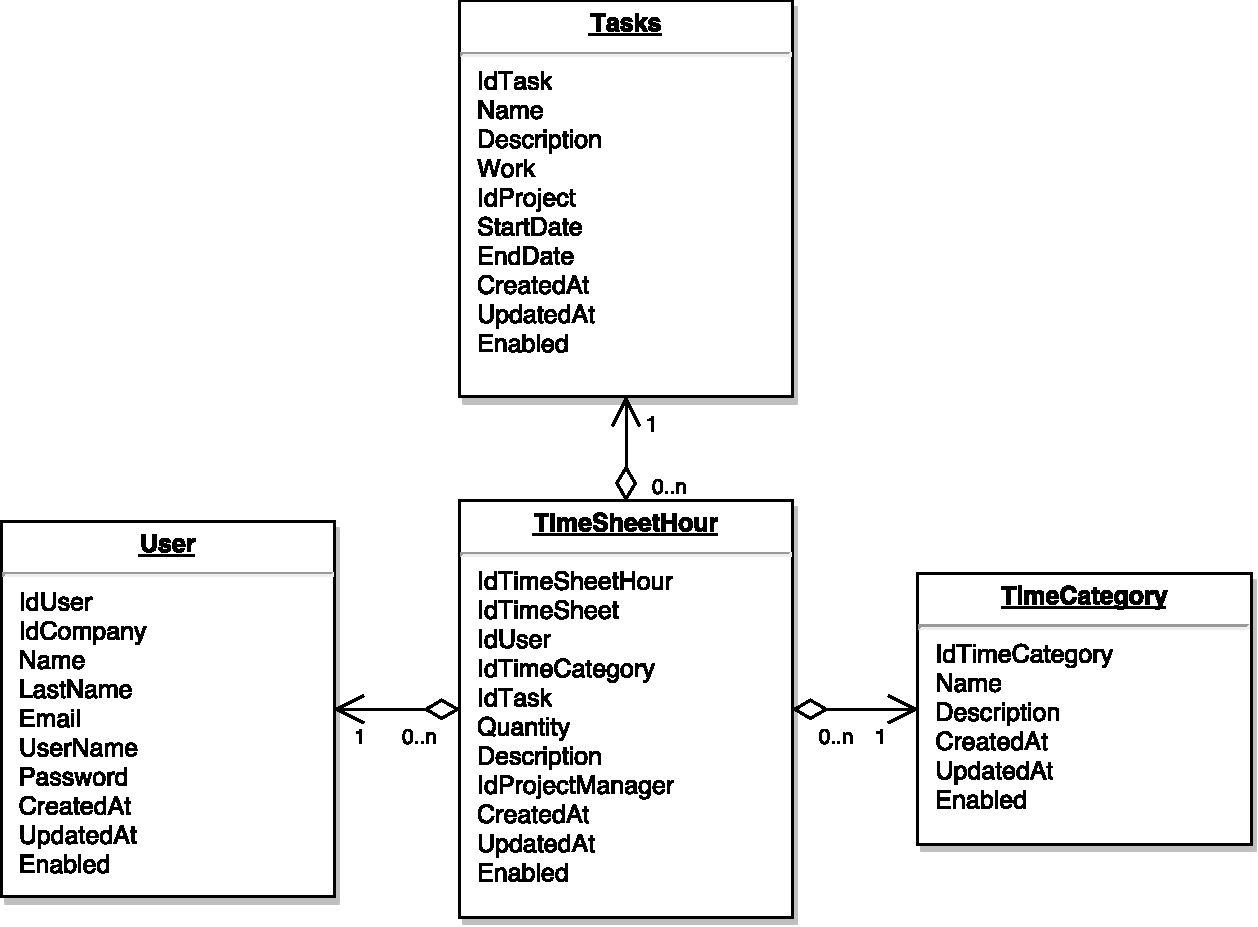
\includegraphics[width=0.8\textwidth]{Bilder/Diagramm.pdf} 
	\caption{Diagramm eines Software Designs}
	\label{fig:Diagramm-DrawIo}
\end{figure}

Ein weiteres kostenloses Tool für die Darstellung von Klassendiagrammen oder auch Sequenzdiagrammen ist \textbf{\href{http://staruml.io/}{StarUML}}. Dieses generiert auch SVG Dateien, welche du mithilfe von Inkscape zu PDF Dateien konvertieren kannst.

%\chapter{Mathematik}

\section{Text}
Hier steht ein beispielhafter Text bei dem nun auf eine sehr bekannte und durchaus vertraute Formel im Text direkt mit $c = \sqrt{a^2 + b^2}$ eingegangen wird. Dabei können auch Winkel wie: $\alpha, \beta, \gamma$ gerne verwendet werden. Weiterhin werden hier nur Formeln im Bereich der $\mathbb{N}$ dargestellt, gerne können diese aber durch Formeln aus diesem Bereich der $\mathbb{R}$ ergänzt werden.

\section{Formeln}
Beachte bei Formeln keine konkreten Werte anzugeben, sondern die Formel stets nur wie in der Literatur nur als Größengleichungen anzugeben.
\begin{align}
	\sum_{n=0}^{\infty}x=b+n\\
	\frac{b*x}{c} = y
\end{align}

Trotz unterschiedlicher Länge kann man die Gleichheitszeichen auf der gleichen Höhe anbringen wie in \autoref{eq:Gleichung1} und \autoref{eq:Gleichung2} dargestellt, zusätzlich kann man diese auch mit Informationen versehen wie in Formel \autoref{eq:Gleichung3} zu sehen.

\begin{align}
	\label{eq:Gleichung1} a + b &= c\\
	\label{eq:Gleichung2} 5c + 3f &= 4h\\ 
	\label{eq:Gleichung3} \overbrace{5y}^{y = 0} + \underbrace{42x}_{x = 1} &= b
\end{align}

\section{Arrays und Matrizen}

\begin{center}
	\(
	\begin{array}{lc|r}
		a&b&c\\
		\hline
		x&y&z\\
		c&a&b
	\end{array}
	\)
\end{center}

\begin{equation}
	\begin{array}{lcl}
		z & = & a \\
		a + b & = & c \\
		f(x,y,z) & = & x + y + z
	\end{array}
\end{equation}

Hier noch ein paar Matrizen Beispiele in \LaTeX{}.

\begin{align}
	\begin{pmatrix}
		a_{11}	& \dots   & a_{1n}\\
		\vdots	& \ddots  & \vdots\\
		a_{n1}	& \dots   & a_{nn}\\
	\end{pmatrix}
	\\[0.4cm]
	\begin{bmatrix} 
		100&250\\
		300&499
	\end{bmatrix}
	\\[0.4cm]
	\begin{Bmatrix} 
		100&250\\
		300&499
	\end{Bmatrix}
	\\[0.4cm]
	\begin{Vmatrix}
		100&250\\
		300&499
	\end{Vmatrix}
\end{align}

\section{Klammern und Kästchen}

\begin{center}
	\( \Vert x\Vert_{p}=
	\left(
	\sum_{i=1}^{n} | x_{i} |^{p}
	\right)^{\frac{1}{p}} \)
\end{center}

\begin{center}
	\( \left.
	\begin{array}{lc|r}
		a&b&c\\
		\hline
		x&y&z\\
		c&a&b
	\end{array}
	\right\}
	\Rightarrow z,b \)
\end{center}

\begin{equation*}
\mbox{
	\boxed{
		\sin^2\varphi+\cos^2\varphi=1
	}
}
\end{equation*}


%\chapter{Programm- bzw. Quellcode}
\section{Quellcode}
Ein wichtiger Punkt ist auch, dass man Quellcode Stücke mit in seinen Praxisbericht einbaut. Hier nun einfach mal ein Beispiel in Form eines kleinen JAVA Codes, welcher aus einer Datei gelesen wird:

\lstinputlisting[
	label=code:algQuersumme,    % Label; genutzt für Referenzen auf dieses Code-Beispiel
	caption=Algorithmus zur Berechnung der Quersumme,
	captionpos=b,               % Position, an der die Caption angezeigt wird t(op) oder b(ottom)
	style=EigenerJavaStyle,     % Eigener Style der vor dem Dokument festgelegt wurde
	firstline=3,                % Zeilennummer im Dokument welche als erste angezeigt wird
	lastline=18                 % Letzte Zeile welche ins LaTeX Dokument übernommen wird
]{Quellcode/Eigenes-Java-File.java}

Zu beachten ist, dass jedes Stück Code kommentiert werden sollte. Was wird in diesem Abschnitt genau durchgeführt. Wo könnten Probleme auftreten und warum wurde dieses Stück hier hinzugefügt.

\vspace*{0.5cm}

\pagebreak
\textbf{EVENT 01} \textit{INIT}
\lstinputlisting[
	label={code:SSCUI-AfterInit},  % Label; genutzt für Referenzen auf dieses Code-Beispiel
	caption={Initialisierung im Programm},
	captionpos=b,               % Position, für die Caption:  t(op) oder b(ottom)
	style=EigenerABAPStyle,     % Eigener Style der vor dem Dokument festgelegt wurde
	firstline=4,                % Zeilennummer im Dokument welche als erste angezeigt wird
	lastline=23                 % Letzte Zeile welche ins LaTeX Dokument übernommen wird
]{Quellcode/Eigenes-ABAP-File.abap}

Es ist auch möglich, innerhalb des Listings \LaTeX{} Befehle zu verwenden. Dazu muss aber eine Escape-Sequenz angegeben werden. Das folgende Beispiel enthält ein Label, auf das dann verwiesen werden wird: Auch hier funktioniert \texttt{\textbackslash{}autoref}: \enquote{In \autoref{code:var_b} wird der Variable \texttt{b} \ldots}.

\begin{lstlisting}[
  style=EigenerJavaStyle,
  captionpos=b,
  caption={Zuweisung von Variablen},
  label={code:basic_block},
  escapeinside={@}{@}]
int a = 10;
@\label{code:var_b}@int b = a + 20;
return;
\end{lstlisting}

\pagebreak
Weitere Programmiersprachen können auch eingebunden werden. Hier mal ein Beispiel in der Programmiersprache Python:
\lstinputlisting[
	label=code:WhileLoop,    % Label; genutzt für Referenzen auf dieses Code-Beispiel
	caption=Algorithmus zum schätzen einer Zahl in Python,
	captionpos=b,               % Position, an der die Caption angezeigt wird t(op) oder b(ottom)
	style=EigenerPythonStyle,   % Eigener Style der vor dem Dokument festgelegt wurde
	firstline=0,                % Zeilennummer im Dokument welche als erste angezeigt wird
	lastline=23                 % Letzte Zeile welche ins LaTeX Dokument übernommen wird
]{Quellcode/Eigenes-Python-File.py}

\clearpage % Absichtlicher Seitenumbruch, um ein besseres Layout zu erhalten.

\section{Pseudocode}
Pseudocode kann hilfreich sein, wenn \enquote{richtig} implementierte Algorithm in einer Programmiersprache zu lang sind und diese mittels Pseudocode bündig zusammengefasst werden können. \autoref{lst:euclid} zeigt Pseudocode.

Die Doku für das Package und damit eine Liste aller Befehle findet sich unter \newline
\url{http://tug.ctan.org/macros/latex/contrib/algorithmicx/algorithmicx.pdf}

\begin{algorithm}
	\caption{Euclid's algorithm}\label{lst:euclid}
	\begin{algorithmic}[1]
		\Procedure{Euclid}{$a,b$}\Comment{The g.c.d. of a and b}
			\State $r\gets a\bmod b$
			\While{$r\not=0$}\Comment{We have the answer if r is 0}
				\State $a\gets b$
				\State $b\gets r$
				\State $r\gets a\bmod b$
			\EndWhile\label{euclidendwhile}
			\State \textbf{return} $b$\Comment{The gcd is b}
		\EndProcedure
	\end{algorithmic}
\end{algorithm}

%\chapter{Literaturhinweise}

\textbf{Hinweis}: Verwendest du eine Quelle nicht, dann nimmt \LaTeX{} diese nicht mit ins Literaturverzeichnis auf!

\section{Fußnoten und Literaturverweise}
Hamburger, Döner, Currywurst\footnote{Hier fehlt eindeutig das Lieblingsessen der Informatiker, die Pizza!} - jeder kennt sie, jeder liebt sie und jeder isst sie.
Weil die Zeit drängt\cite{Bonnen.2016}, der Hunger groß ist und der nächste Schnellimbiss\cite{Forsthuber.2016} nur drei Schritte voraus. Und nach dem Essen?
Sind wir zwar satt, aber meist nicht wirklich glücklich, weil Fastfood\cite{Friedl.2017} meist eben auch nicht wirklich gut ist \cite{Kuhnlein.2016}.

Ja, uns ist bewusst, dass die Literatur nicht zum Text passt.
Deswegen hier nochmals der Rest.\cite{Mukherjee.2017, Preuss.2017, Schell.2017, Smith.2017, Visser.2017, Zaidi.2017, o.V..o.J.}

Übrigens: \acfp{ISBN} gehören nicht in die Bibliographie und werden deshalb auch nicht angezeigt.


% ---- Literaturverzeichnis
\cleardoublepage
\renewcommand*{\chapterpagestyle}{plain}
\pagestyle{plain}
\pagenumbering{Roman}                   % Römische Seitenzahlen
\setcounter{page}{\numexpr\value{savepage}+1}
\printbibliography[title=Literaturverzeichnis]

% ---- Anhang
\appendix
%\clearpage
%\pagenumbering{Roman}  % römische Seitenzahlen für Anhang

\newpage
\end{document}
